\documentclass[a4paper]{article}\usepackage[]{graphicx}\usepackage[]{color}
% maxwidth is the original width if it is less than linewidth
% otherwise use linewidth (to make sure the graphics do not exceed the margin)
\makeatletter
\def\maxwidth{ %
  \ifdim\Gin@nat@width>\linewidth
    \linewidth
  \else
    \Gin@nat@width
  \fi
}
\makeatother

\definecolor{fgcolor}{rgb}{0.345, 0.345, 0.345}
\newcommand{\hlnum}[1]{\textcolor[rgb]{0.686,0.059,0.569}{#1}}%
\newcommand{\hlstr}[1]{\textcolor[rgb]{0.192,0.494,0.8}{#1}}%
\newcommand{\hlcom}[1]{\textcolor[rgb]{0.678,0.584,0.686}{\textit{#1}}}%
\newcommand{\hlopt}[1]{\textcolor[rgb]{0,0,0}{#1}}%
\newcommand{\hlstd}[1]{\textcolor[rgb]{0.345,0.345,0.345}{#1}}%
\newcommand{\hlkwa}[1]{\textcolor[rgb]{0.161,0.373,0.58}{\textbf{#1}}}%
\newcommand{\hlkwb}[1]{\textcolor[rgb]{0.69,0.353,0.396}{#1}}%
\newcommand{\hlkwc}[1]{\textcolor[rgb]{0.333,0.667,0.333}{#1}}%
\newcommand{\hlkwd}[1]{\textcolor[rgb]{0.737,0.353,0.396}{\textbf{#1}}}%
\let\hlipl\hlkwb

\usepackage{framed}
\makeatletter
\newenvironment{kframe}{%
 \def\at@end@of@kframe{}%
 \ifinner\ifhmode%
  \def\at@end@of@kframe{\end{minipage}}%
  \begin{minipage}{\columnwidth}%
 \fi\fi%
 \def\FrameCommand##1{\hskip\@totalleftmargin \hskip-\fboxsep
 \colorbox{shadecolor}{##1}\hskip-\fboxsep
     % There is no \\@totalrightmargin, so:
     \hskip-\linewidth \hskip-\@totalleftmargin \hskip\columnwidth}%
 \MakeFramed {\advance\hsize-\width
   \@totalleftmargin\z@ \linewidth\hsize
   \@setminipage}}%
 {\par\unskip\endMakeFramed%
 \at@end@of@kframe}
\makeatother

\definecolor{shadecolor}{rgb}{.97, .97, .97}
\definecolor{messagecolor}{rgb}{0, 0, 0}
\definecolor{warningcolor}{rgb}{1, 0, 1}
\definecolor{errorcolor}{rgb}{1, 0, 0}
\newenvironment{knitrout}{}{} % an empty environment to be redefined in TeX

\usepackage{alltt}
\usepackage[left=2.5cm,top=3cm,bottom=3.5cm,right=2.5cm]{geometry} % Ajustar Margenes
\usepackage[spanish, es-tabla, es-nodecimaldot]{babel} % para producir la letras acentuadas "?"
\usepackage[utf8]{inputenc} % ecribir acentos ?
\usepackage{booktabs} % Para crear tablas
\usepackage{graphicx} % Para manipular imagenes 
\usepackage{amsmath} % Para el manejo de ecuaciones
\usepackage{color} % Para los colores
\usepackage{hyperref}
\hypersetup{colorlinks=true, linkcolor=blue, filecolor=magenta, urlcolor=blue}
\title{Resultados} % Agregar titulo
\author{Rafael Eduardo Diaz} % Agregar Nombre

\setlength{\abovecaptionskip}{2pt plus 1pt minus 0pt} % Chosen fairly arbitrarily



\IfFileExists{upquote.sty}{\usepackage{upquote}}{}
\begin{document}

\maketitle
\section{Aplicación}

A continuación, ilustramos todos los modelos descritos anteriormente aplicándolos a dos conjuntos de datos, para la serie anual del número de homicidios en Colombia de 1960 a 2018 se ajustaron varios PHMM, mientras que para la serie mensual de incendios forestales en Colombia, entre el 2002 y 2016 se ajustaron diversos ZIP-HMM. Antes de que se ajusten los modelos, se llevo a cabo un análisis exploratorio básico del conjunto de datos que aborda algunos problemas que generalmente se presentan al visualizar los datos de conteo. Al final de la sección, se comparan todos los modelos ajustados, tanto desde el enfoque clásico como Bayesiano, y se selecciona el mejor modelo a partir de las dos metodologías. 

\vspace{5mm} %5mm vertical space

Para ambas series, la aplicación de modelos estándar como modelos auto regresivos de media móvil (ARMA) sería inapropiado, ya que estos modelos se basan en la distribución normal. En cambio, se propone un modelo usual para datos con conteos la distribución de Poisson, pero, como se demostrará más adelante, las series presenta una sobredispersión considerable con respecto a la distribución de Poisson, y fuerte dependencia serial positiva además de inflación en ceros en el caso de la serie de incendios. Por lo tanto, un modelo que consiste en variables aleatorias independientes de Poisson; sería por dos razones inadecuado. Primero que puede haber algunos períodos con una baja tasa de homicidios e incendios, y algunos con una tasa relativamente alta. Los HMMs, permiten que la distribución de probabilidad de cada observación dependa del estado no observado (u oculto) de una cadena de Markov, por lo tanto puede acomodar la sobredispersión y la dependencia serial al mismo tiempo.



\subsection{Descripción de los datos}

\textbf{Homicidios:} Esta tabla contiene las cifras actualizadas de homicidios en Colombia 1960-2018, con base en la Compilación de estadísticas históricas económicas y sociales, extraída del \href{https://www.dnp.gov.co/estudios-y-publicaciones/estudios-economicos/Paginas/estadisticas-historicas-de-colombia.aspx}{departamento Nacional de Planeación} (DNP) se consulto específicamente el capítulo 8 indicadores de violencia, se complemento junto con las estadísticas delectivas de la \href{https://www.policia.gov.co/grupo-información-criminalidad/estadistica-delictiva}{Policía Nacional} y Medicina Legal. Los datos publicados corresponden a consolidados de los Delitos de Impacto del país, así mismo la Actividad Operativa realizada por la Policía Nacional. Mientras que para la población total Colombiana se extrajo la información de la sección Estadísticas por tema, demografía y población. La serie es anual para un total de 59 observaciones y se expresa como el número de homicidios por cada 100.000 habitantes comunmente conocida como \emph{Tasa de homicidios}, para ser posible la modelación se redondeo la cifra al entero más cercano. Nota: La confiabilidad de los datos de la tasa de asesinatos puede variar, de acuerdo a la fuente.

% latex table generated in R 3.6.0 by xtable 1.8-4 package
% Sun Jul 14 00:13:40 2019
\begin{table}[ht]
\centering
\begin{tabular}{rrrrrrrrrrrrrrrrrrrr}
  \hline
  \hline
31 & 31 & 31 & 32 & 31 & 32 & 30 & 29 & 31 & 19 & 21 & 23 & 23 & 23 & 24 & 24 & 25 & 27 & 26 & 27 \\ 
  29 & 36 & 34 & 30 & 30 & 40 & 48 & 52 & 63 & 65 & 68 & 78 & 76 & 74 & 70 & 66 & 68 & 62 & 58 & 61 \\ 
  65 & 49 & 69 & 56 & 48 & 42 & 40 & 39 & 36 & 35 & 34 & 32 & 32 & 32 & 27 & 26 & 25 & 25 & 25 &  \\ 
   \hline
\end{tabular}
\caption{Número de homicidios por 100.000 habitantes en Colombia, 1960 - 2018.} 
\end{table}


\vspace{5mm} %5mm vertical space

\textbf{Incendios:} Los datos referentes a incendios forestales en Colombia, fueron recolectados de la página del IDEAM - Instituto de Hidrología, Meteorología y Estudios Ambientales que ha venido realizando una revisión histórica y consolidado de los datos reportados por las siguientes instituciones: entidades del SINA, entidades del Sistema Nacional para la Prevención y atención de Desastres, la Defensa Civil, entre otras, y aunque se ha adoptado un Formulario Único de Captura (MAVDT \& otros, 2002), con el fin de estandarizar la información, este no ha sido utilizado en su totalidad y existen otros formatos desarrollados por las distintas entidades, de acuerdo con sus particularidades técnicas e informáticas, lo que ha dificultado la estandarización en el flujo de información.
\\
Las estadísticas sobre incendios en Colombia, permiten en términos generales, realizar análisis de su comportamiento bajo diferentes escenarios, esto es, por regiones, departamentos o municipios, con Niño o en condiciones climáticas normales,  por cobertura vegetal afectada, por Corporación Autónoma Regional, por año o por mes, y de esta manera, poder ser  utilizarlas para priorizar áreas, orientar acciones o sustentar la necesidad de realizar estudios más detallados. El Ideam ha venido realizando una revisión histórica de los datos reportados por las instituciones anteriormente mencionadas, con el fin de tener datos más confiables que permitan tener una mejor aproximación al tema. La variable de interés es el número de grandes incendios forestales (GIF), y se definen como aquellos incendios que superan las 500 hectáreas forestales afectadas. El número de observaciones es mensual iniciando en enero del 2002 y finalizando en diciembre del 2016, para un total 180 observaciones.



% latex table generated in R 3.6.0 by xtable 1.8-4 package
% Sun Jul 14 00:13:40 2019
\begin{table}[ht]
\centering
\begin{tabular}{rrrrrrrrrrrrr}
  \hline
 & Jan & Feb & Mar & Apr & May & Jun & Jul & Aug & Sep & Oct & Nov & Dec \\ 
  \hline
2002 &  10 &   8 &  12 &   2 &   0 &   1 &   0 &   6 &   1 &   1 &   0 &   0 \\ 
  2003 &   5 &   6 &  11 &   3 &   0 &   0 &   5 &   0 &   3 &   0 &   0 &   0 \\ 
  2004 &   7 &  14 &  10 &   1 &   0 &   0 &   3 &  12 &   4 &   1 &   0 &   3 \\ 
  2005 &   5 &   6 &  13 &   4 &   1 &   0 &   4 &   9 &  25 &   1 &   0 &   2 \\ 
  2006 &   2 &   3 &   0 &   0 &   0 &   0 &   6 &   6 &  10 &   0 &   0 &   0 \\ 
  2007 &  19 & 100 &  16 &   1 &   1 &   0 &   0 &   0 &   1 &   0 &   1 &   0 \\ 
  2008 &   3 &   4 &   3 &   1 &   0 &   0 &   0 &   0 &   0 &   0 &   0 &   0 \\ 
  2009 &   1 &   6 &   5 &   3 &   3 &   3 &  12 &  24 &  58 &  22 &   0 &   7 \\ 
  2010 & 103 &  95 &  37 &   3 &   0 &   0 &   0 &   0 &   0 &   0 &   0 &   0 \\ 
  2011 &  14 &  21 &   3 &   0 &   0 &   1 &   2 &  16 &  20 &   0 &   0 &   0 \\ 
  2012 &  16 &  27 &  14 &   1 &   3 &   3 &  31 &  36 &  45 &   4 &   3 &   3 \\ 
  2013 &  62 &  56 &  33 &  14 &   0 &   1 &  19 &  17 &  36 &  13 &   2 &   0 \\ 
  2014 &  15 &  32 &  18 &  17 &   2 &   0 &  48 &  38 &  47 &   3 &   1 &   0 \\ 
  2015 &  18 &  19 &  27 &   4 &   9 &   5 &  11 &  31 &  39 &  12 &   0 &   8 \\ 
  2016 &  40 &  60 &  58 &  12 &   0 &   0 &   5 &  22 &  18 &   1 &   0 &   2 \\ 
   \hline
\end{tabular}
\caption{Número de Grandes Incendios Forestales (GIF) en Colombia, 2002 - 2016.} 
\end{table}


\subsubsection*{Estadísticas de resumen}

A continuación se muestran algunas estadísticas descriptivas, sobre la serie de homicidios Colombia para los años 1960-2018.


\begin{table}[!htbp] \centering 
  \caption{Estadísticas de Resumen serie homicidios en Colombia.} 
  \label{} 
\begin{tabular}{@{\extracolsep{5pt}}lcccccccc} 
\\[-1.8ex]\hline 
\hline \\[-1.8ex] 
Statistic & \multicolumn{1}{c}{N} & \multicolumn{1}{c}{Mean} & \multicolumn{1}{c}{St. Dev.} & \multicolumn{1}{c}{Min} & \multicolumn{1}{c}{Pctl(25)} & \multicolumn{1}{c}{Median} & \multicolumn{1}{c}{Pctl(75)} & \multicolumn{1}{c}{Max} \\ 
\hline \\[-1.8ex] 
Homicidios & 59 & 14,189.170 & 8,012.999 & 3,908 & 5,969.5 & 12,626 & 20,907 & 28,837 \\ 
Tasa & 59 & 40.421 & 17.111 & 19.256 & 27.057 & 32.359 & 53.894 & 77.946 \\ 
\hline \\[-1.8ex] 
\end{tabular} 
\end{table} 


En la tabla el número mínimo de homicidios ocurrido en este período fue de 3908 con una Tasa de 19.26 homicidios por cada 100.000 habitantes, que corresponde al año 1969, mientras que el máximo número de homicidios registrados fue de 28.837 en el año 2002, sin embargo la Tasa más alta de homicidios fue en el año 1991 con casi 78 homicidios por cada 100.000 la más alta de la región para esta época según un estudio que presentó la CEPAL encontró que la tasa promedio homicidios en Latino-américa era de 20 por cada 100.000 habitantes. Algunas investigaciones sobre el tema como la de Franco (2006) y Pécaut (2003) han enfatizado ciertos aspectos coyunturales, tales como el problema del narcotráfico, la persistencia del conflicto armado interno, la debilidad del Estado, la corrupción y la inmadurez en el ejercicio de la ciudadanía pero aun son insuficientes los estudios y poco el consenso sobre las explicaciones de fondo de la situación de violencia que vive el país
\\
En el conjunto de los países con conflictos armados en el mundo, Colombia presenta uno de los más altos índices de homicidio40/100.000 en estas últimas seis décadas, con cifras comparables a las de países con guerra civil declarada. (Franco, 1980).

\begin{knitrout}
\definecolor{shadecolor}{rgb}{0.91, 0.91, 0.91}\color{fgcolor}\begin{figure}
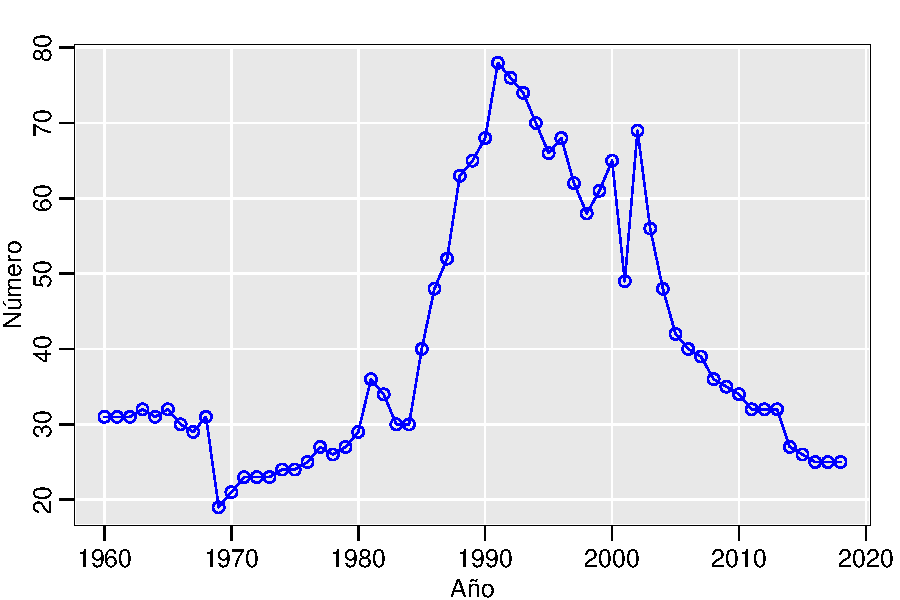
\includegraphics[width=\maxwidth]{figure/unnamed-chunk-7-1} \caption[Serie de tiempo homicidios en Colombia desde el año 1960 hasta el año 2018]{Serie de tiempo homicidios en Colombia desde el año 1960 hasta el año 2018.}\label{fig:unnamed-chunk-7}
\end{figure}


\end{knitrout}

En la figura 2, se encuentra gráficada la densidad de la serie Tasa de homicidios por 100.000 habitantes en Colombia, se deduce que utilizar modelo de regresión Poisson, sería inapropiado pues parece haber una mixtura entre dos distribuciones, ahora la pregunta que deberíamos hacernos es si estas dos distribuciones están correlacionadas, pues de no estarlo una opción para modelar esta serie sería utilizar una mixtura entre dos o más distribuciones independientes, como se muestra en Zucchini (2012, capítulo 1). Por otra parte parece haber una sobredispersión enorme pues mientras la media se sitúa en 40, la varianza es 292 es decir 7 veces la media, y recordemos que para la distribución Poisson $\mu = \sigma^2 = \lambda$. 

Un primer período de incremento acelerado que va desde comienzos de los 80, en particular desde 1983, hasta 1991. Es la fase más crítica de violencia, en particular de violencia homicida, en los anales de la ciudad. Las tasas de homicidio en la ciudad llegaron a marcar la tendencia de la curva de homicidios a nivel nacional. Investigaciones anteriores \textbf{19-22} han tratado de explicar este incremento acelerado mediante la convergencia de los problemas acumulados de debilidad institucional, ausencias estatales, ciudadanía precaria, desempleo e inequidades crecientes, con la expansión del fenómeno del narcotráfico en la ciudad \textbf{23} y su confrontación armada estatal, con la intensificación de la presencia urbana del conflicto armado interno, en especial la actuación de las milicias afines a las organizaciones guerrilleras y la emergencia y acelerado desarrollo de organizaciones paramilitares \textbf{24,25}.

\begin{knitrout}
\definecolor{shadecolor}{rgb}{0.91, 0.91, 0.91}\color{fgcolor}\begin{figure}
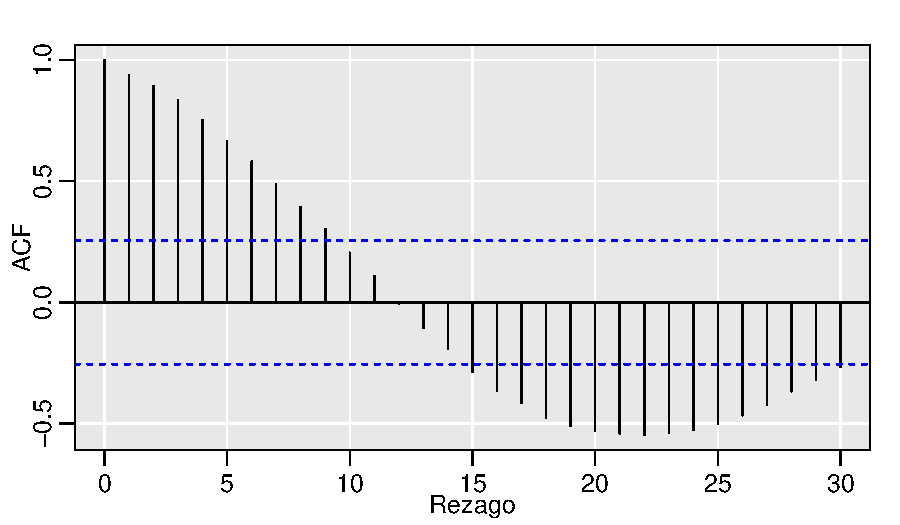
\includegraphics[width=\maxwidth]{figure/unnamed-chunk-8-1} \caption[Función de autocorrelación muetral, y kernel de densidad para la serie homicidios en Colombia (1960-2018)]{Función de autocorrelación muetral, y kernel de densidad para la serie homicidios en Colombia (1960-2018).}\label{fig:unnamed-chunk-8}
\end{figure}


\end{knitrout}

En la figura 3 se observa la función de autocorrelación muestral para la serie Tasa de homicidios hasta el rezago 30, como se evidencia existe una fuerte dependencia serial en los datos por lo que seria inapropiado utilizar un modelo de mixturas independientes (distribución Poisson), como alternativa surge la utilización de los modelos ocultos de Markov, en este caso se utilizara un PHMM.


\subsubsection*{Ajuste clásico PHMM}





Primero ajustamos varios modelos Poisson ocultos de Markov con 1 a 5 estados, y tres modelos con mixturas independientes con 2, 3 y 4 componentes de la distribución Poisson utilizando el paquete \textbf{flexmix} de R. Por último registramos los siguientes valores en la Tabla 3, el número de parámetros estimados, la log-verosimilitud el criterio de información de Akaike (AIC) y el criterio de información bayesiano (BIC). Con el fin de seleccionar el modelo más apropiado, el valor que minimiza el AIC es el PHMM de orden 3 con un valor de 404.02, mientras que el BIC indica que el modelo apropiado es un PHMM de orden 2, con un valor de 418.96. Tanto el BIC y AIC resuelven este problema mediante la introducción de un término de penalización para el número de parámetros en el modelo, el término de penalización es mayor en el BIC que en el AIC. El BIC generalmente penaliza parámetros libres con más fuerza que hace el criterio de información de Akaike, aunque depende del tamaño de $n$ y la magnitud relativa de $n$ y $p$. Como el tamaño de la muestra es relativamente grande $n = 59$, y la cantidad de parámetros que se estiman en un HMM es bastante utilizaremos el BIC en este caso en concreto, eligiendo por tanto el PHMM de orden 2.

% latex table generated in R 3.6.0 by xtable 1.8-4 package
% Sun Jul 14 00:13:43 2019
\begin{table}[ht]
\centering
\begin{tabular}{rlrrrr}
  \hline
 & Modelo & p & logL & AIC & BIC \\ 
  \hline
1 & PHMM - 1 Estado &   1 & -356.91 & 715.81 & 717.89 \\ 
  2 & PHMM - 2 Estados &   4 & -201.32 & 410.65 & 418.96 \\ 
  3 & PHMM - 3 Estados &   9 & -193.01 & 404.02 & 422.71 \\ 
  4 & PHMM - 4 Estados &  16 & -190.84 & 413.69 & 446.93 \\ 
  5 & PHMM - 5 Estados &  25 & -190.29 & 430.58 & 482.51 \\ 
  6 & mixtura indep. (2) &   3 & -229.38 & 464.75 & 470.98 \\ 
  7 & mixtura indep. (3) &   5 & -228.11 & 466.21 & 476.60 \\ 
  8 & mixtura indep. (4) &   7 & -228.11 & 472.69 & 487.23 \\ 
   \hline
\end{tabular}
\caption{Datos homicidios: comparación de modelos ocultos de Markov (estacionarios) por AIC y BIC.} 
\end{table}


\begin{knitrout}
\definecolor{shadecolor}{rgb}{0.91, 0.91, 0.91}\color{fgcolor}\begin{figure}[h]
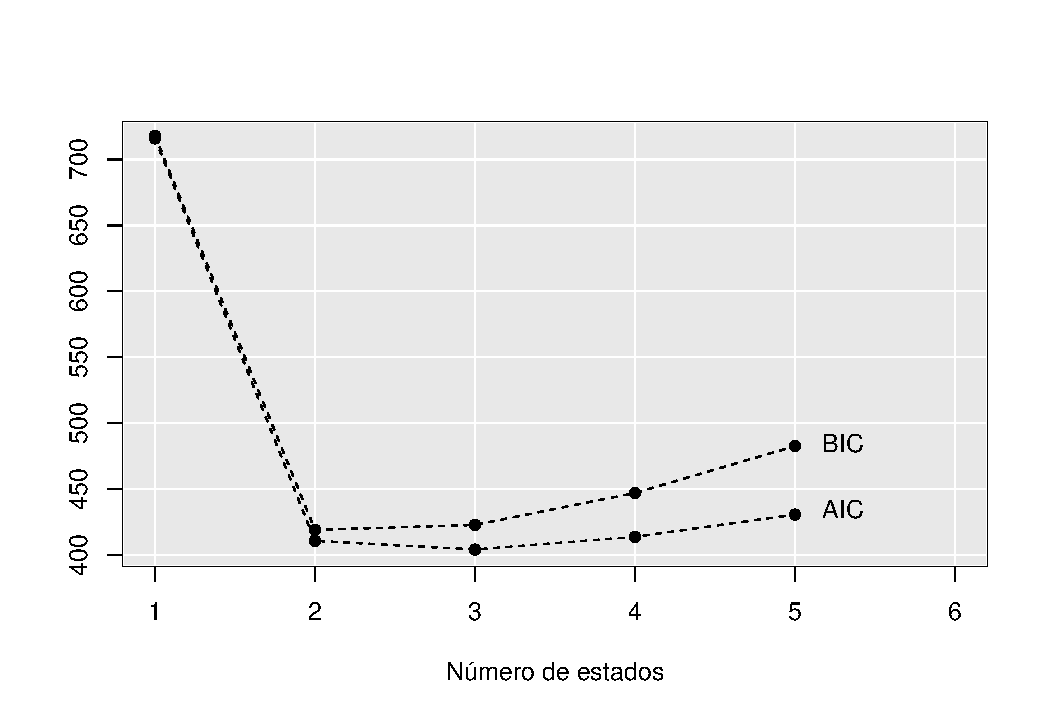
\includegraphics[width=\maxwidth]{figure/unnamed-chunk-12-1} \caption[Serie homicidios]{Serie homicidios: selección de modelos AIC y BIC.}\label{fig:unnamed-chunk-12}
\end{figure}


\end{knitrout}

Varios comentarios surgen de la Tabla 4. En primer lugar, dada la dependencia en serie manifestada en la Figura 2, no es sorprendente que los modelos de mezcla independientes no tengan un buen desempeño en relación con los HMM. En segundo lugar, aunque quizás sea obvio a priori que ni siquiera se debe intentar establecer un modelo con un máximo de 16 o 25 parámetros para 59 observaciones, y observaciones dependientes, es interesante explorar las funciones de verosimilitud en el caso de HMM con cuatro y cinco estados. La verosimilitud parece ser altamente multimodal en estos casos, y es fácil encontrar varios máximos locales utilizando diferentes valores de inicio. Una estrategia que parece tener éxito en estos casos es comenzar todas las probabilidades de transición fuera de la diagonal en valores pequeños (como 0.1 o 0.05), mientras que para los valores de las medias estado dependientes se pueden usar los valores de los deciles, calculados a partir de la variable de interés.



La estimaciones del PHMM de dos estados se muestran a continuación, primero la tpm $A$, además del vector de medias de los estados dependientes $\lambda$ y los valores de la distribución estacionaria $\pi$. 

$$
A = \begin{pmatrix}{}
  0.980 & 0.020 \\ 
  0.064 & 0.936 \\ 
\end{pmatrix}
$$

$$\lambda = (29.715, 62.812) \ \ \ \ \pi = (0.764, 0.235)$$

Ahora miraremos otras metodologías alternativas a los criterios de información AIC y BIC, que determinan si el modelo tiene un buen ajuste. Entre estas es útil comparar las funciones de autocorrelación de los HMM con dos, tres, cuatro y cinco estados con la función de autocorrelación muestral (ACF). Los ACF de los modelos se pueden encontrar utilizando la función `Bayeshmmcts::pois.HMM.moments` utilizando la ecuación de Zucchini, pág. 55. En forma tabular los ACF se muestran en la tabla 5:

% latex table generated in R 3.6.0 by xtable 1.8-4 package
% Sun Jul 14 00:13:43 2019
\begin{table}[ht]
\centering
\begin{tabular}{rrrrrrrrrrrrr}
  \hline
 & 1 & 2 & 3 & 4 & 5 & 6 & 7 & 8 & 9 & 10 & 11 & 12 \\ 
  \hline
observaciones & 0.94 & 0.89 & 0.83 & 0.75 & 0.66 & 0.58 & 0.49 & 0.39 & 0.30 & 0.20 & 0.11 & -0.00 \\ 
  PHMM 2 Estados & 0.77 & 0.71 & 0.65 & 0.59 & 0.54 & 0.50 & 0.46 & 0.42 & 0.38 & 0.35 & 0.32 & 0.29 \\ 
  PHMM 3 Estados & 0.79 & 0.75 & 0.71 & 0.68 & 0.64 & 0.61 & 0.58 & 0.55 & 0.52 & 0.50 & 0.47 & 0.45 \\ 
  PHMM 4 Estados & 0.80 & 0.76 & 0.72 & 0.69 & 0.65 & 0.62 & 0.58 & 0.55 & 0.52 & 0.50 & 0.47 & 0.44 \\ 
   \hline
\end{tabular}
\caption{Datos homicidios: ACF y ACF de los cuatro modelos hasta el rezago 12.} 
\end{table}


\begin{knitrout}
\definecolor{shadecolor}{rgb}{0.91, 0.91, 0.91}\color{fgcolor}\begin{figure}[h]
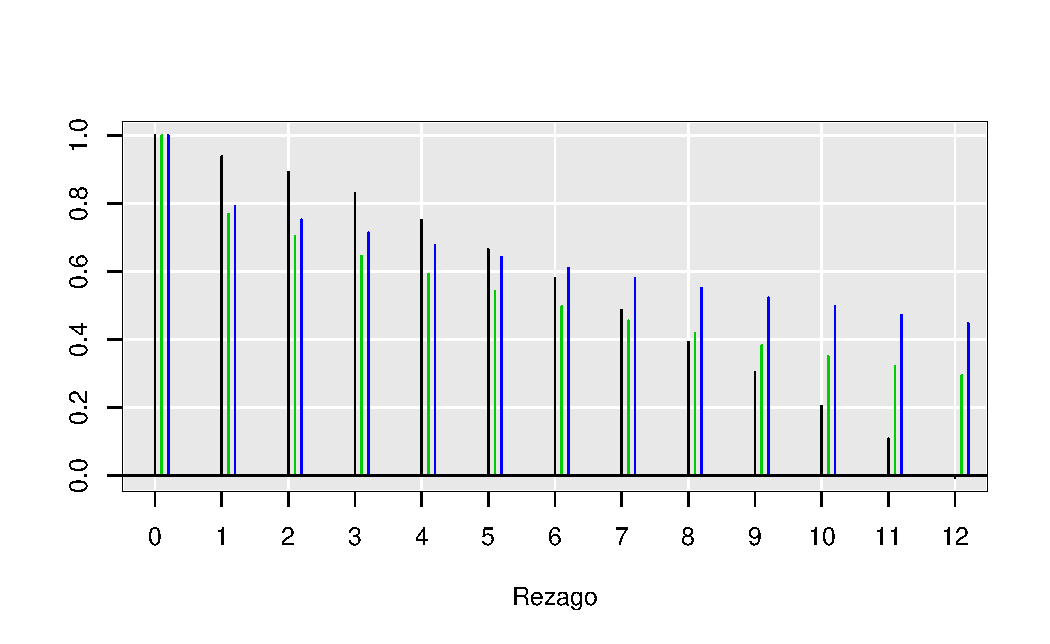
\includegraphics[width=\maxwidth]{figure/unnamed-chunk-15-1} \caption[Datos homicidios]{Datos homicidios: ACF y ACF de los PHMM con dos y tres estados.}\label{fig:unnamed-chunk-15}
\end{figure}


\end{knitrout}

En la Figura 6, de izquierda a derecha se muestran el ACF de las observaciones, la barra de color verde pertenece al modelo de dos estados y la azul al modelo de tres estados. Nos interesa ver como está yuxtapuesto los ACF de ambos modelos con respecto al ACF de las observaciones. Está claro que los ACF del modelo con tres estados corresponden bien con el ACF de las observaciones hasta aproximadamente el rezago 6, mientras que el modelo 2 estados coincide hasta el rezago 9. Sin embargo, se pueden aplicar diagnósticos más sistemáticos, como se mostrará a continuación.

\subsubsection*{Verificación de supuestos del PHMM}

En este caso hemos elegido el BIC como criterio para la selección del mejor modelo como mostramos anteriormente, sin embargo sigue existiendo el problema de decidir si el modelo es realmente adecuado; por lo tanto se necesitan herramientas para evaluar la bondad general del ajuste del modelo e identificar valores atípicos en relación con el modelo. En el contexto más simple como por ejemplo los modelos de regresión (teoría normal), el papel que juegan los residuales como herramienta para la verificación del supuesto del modelo está muy bien establecido, entre estos supuestos están la normalidad de los residuales, la homocedasticidad y la independencia de estos. Los pseudo-residuos (también conocidos como residuos quantílicos) que se ilustraron en la sección tres tienen la intención de cumplir esta función de manera mucho más general, y que son útiles en el contexto de los HMM. 

\begin{knitrout}
\definecolor{shadecolor}{rgb}{0.91, 0.91, 0.91}\color{fgcolor}\begin{figure}[h]
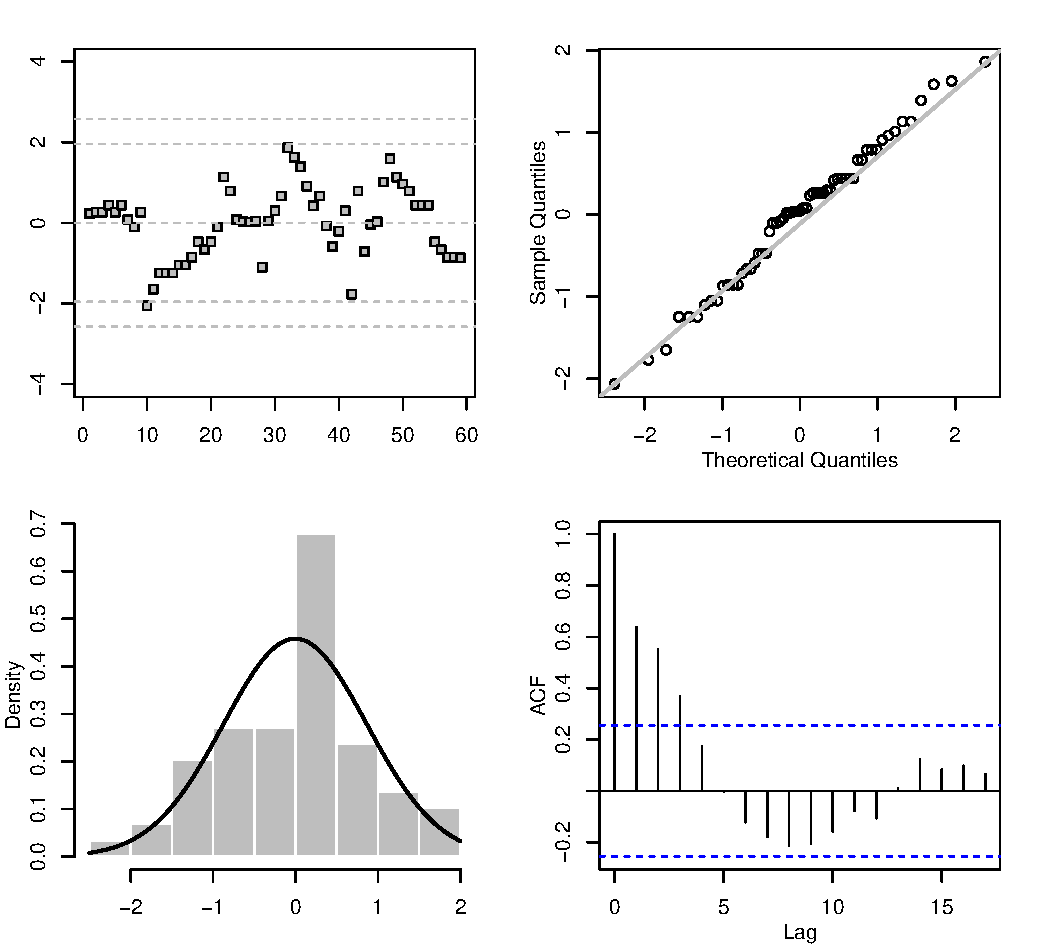
\includegraphics[width=\maxwidth]{figure/unnamed-chunk-16-1} \caption[Grafico pseudo-residuales ordinarios para el PHMM de 2 estados]{Grafico pseudo-residuales ordinarios para el PHMM de 2 estados.}\label{fig:unnamed-chunk-16}
\end{figure}


\end{knitrout}

En el gráfico 6, se muestra los pseudo residuales ordinarios del PHMM con 2 estados. La fila superior izquierda muestra el diagramas de índice de los pseudo-residuos normales, con líneas horizontales en 0, $\pm 1.96$ y $\pm 2.58$. En la parte superior derecha se muestra los gráficos de cuantiles-cuantiles de los pseudo-residuos normales, con los cuantiles teóricos en el eje $x$. La última fila muestra en la parte izquierda el histograma de los pseudo residuales normales, y en la parte derecha la función de autocorrelación muestral de los pseudo-residuos normales. Efectivamente los pseudo-residuales parecen distribuirse normalmente, sin embargo realizamos la prueba de Shapiro-Wilks para verificar este supuesto, donde el p-valor es 0.7529, por lo tanto no podemos rechazar la hipótesis nula $H_0$, y concluimos que hay suficiente evidencia estadística para decir que los pseudo-residuos se distribuyen normalmente con un nivel de confianza del 95\%. Además todos los puntos están dentro de las bandas de confianza, sin embargo el histograma no parece acomodarse en todos sus puntos a la curva de la distribución normal, y el mayor problema es que los pseudo-residuales parecen estar correlacionados, hasta el rezago 3.

\subsubsection*{Algoritmo Viterbi}

El algoritmo Viterbi, permite realizar la decodificación global de los estados clasificando a cada una de las observaciones en su correspondiente estado, indicando la secuencia más probable de los estados ocultos. Para la serie homicidios de 59 observaciones, el algoritmo Viterbi clasifico 40 observaciones en el estado 1 y 19 en el estado 2. En la grafica 5 se visualiza el algoritmo viterbi, y las distribuciones marginales para cada estado.
\\
La decodificación global (algoritmo Viterbi) es el objetivo principal en muchas aplicaciones, especialmente cuando existen interpretaciones importantes para los estados. Sin embargo los estados no observados en el modelo, no siemprre necesitan tener interpretaciones sustantiva, pues se consideran artefactos útiles para adaptarse a la heterogeneidad no explicada y la dependencia serial de los datos. En el caso de la serie homicidios no parce haber una interpretación clara de los estados.

% latex table generated in R 3.6.0 by xtable 1.8-4 package
% Sun Jul 14 00:13:44 2019
\begin{table}[ht]
\centering
\begin{tabular}{rrrrrrrrrrrrrrrrrrrr}
  \hline
  \hline
1 & 1 & 1 & 1 & 1 & 1 & 1 & 1 & 1 & 1 & 1 & 1 & 1 & 1 & 1 & 1 & 1 & 1 & 1 & 1 \\ 
  1 & 1 & 1 & 1 & 1 & 1 & 2 & 2 & 2 & 2 & 2 & 2 & 2 & 2 & 2 & 2 & 2 & 2 & 2 & 2 \\ 
  2 & 2 & 2 & 2 & 2 & 1 & 1 & 1 & 1 & 1 & 1 & 1 & 1 & 1 & 1 & 1 & 1 & 1 & 1 &  \\ 
   \hline
\end{tabular}
\caption{Resultados de la decodificación global con el algoritmo Viterbi.} 
\end{table}


\begin{knitrout}
\definecolor{shadecolor}{rgb}{0.91, 0.91, 0.91}\color{fgcolor}\begin{figure}
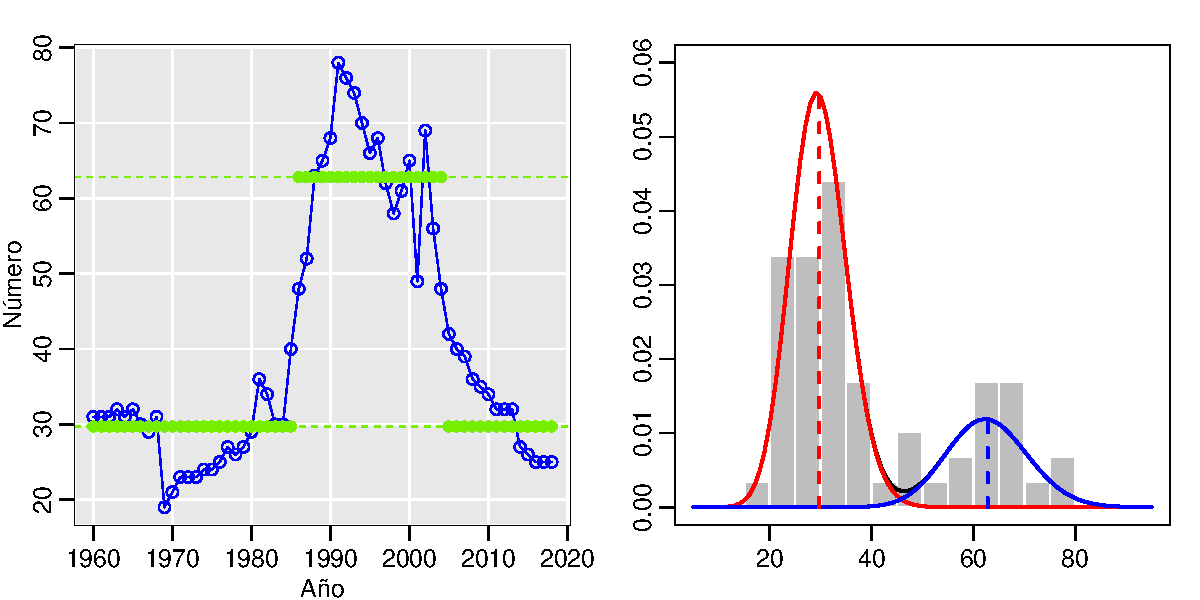
\includegraphics[width=\maxwidth]{figure/unnamed-chunk-18-1} \caption[Algoritmo Viterbi aplicado a un PHMM de dos estados]{Algoritmo Viterbi aplicado a un PHMM de dos estados.}\label{fig:unnamed-chunk-18}
\end{figure}


\end{knitrout}

\begin{knitrout}
\definecolor{shadecolor}{rgb}{0.91, 0.91, 0.91}\color{fgcolor}\begin{figure}
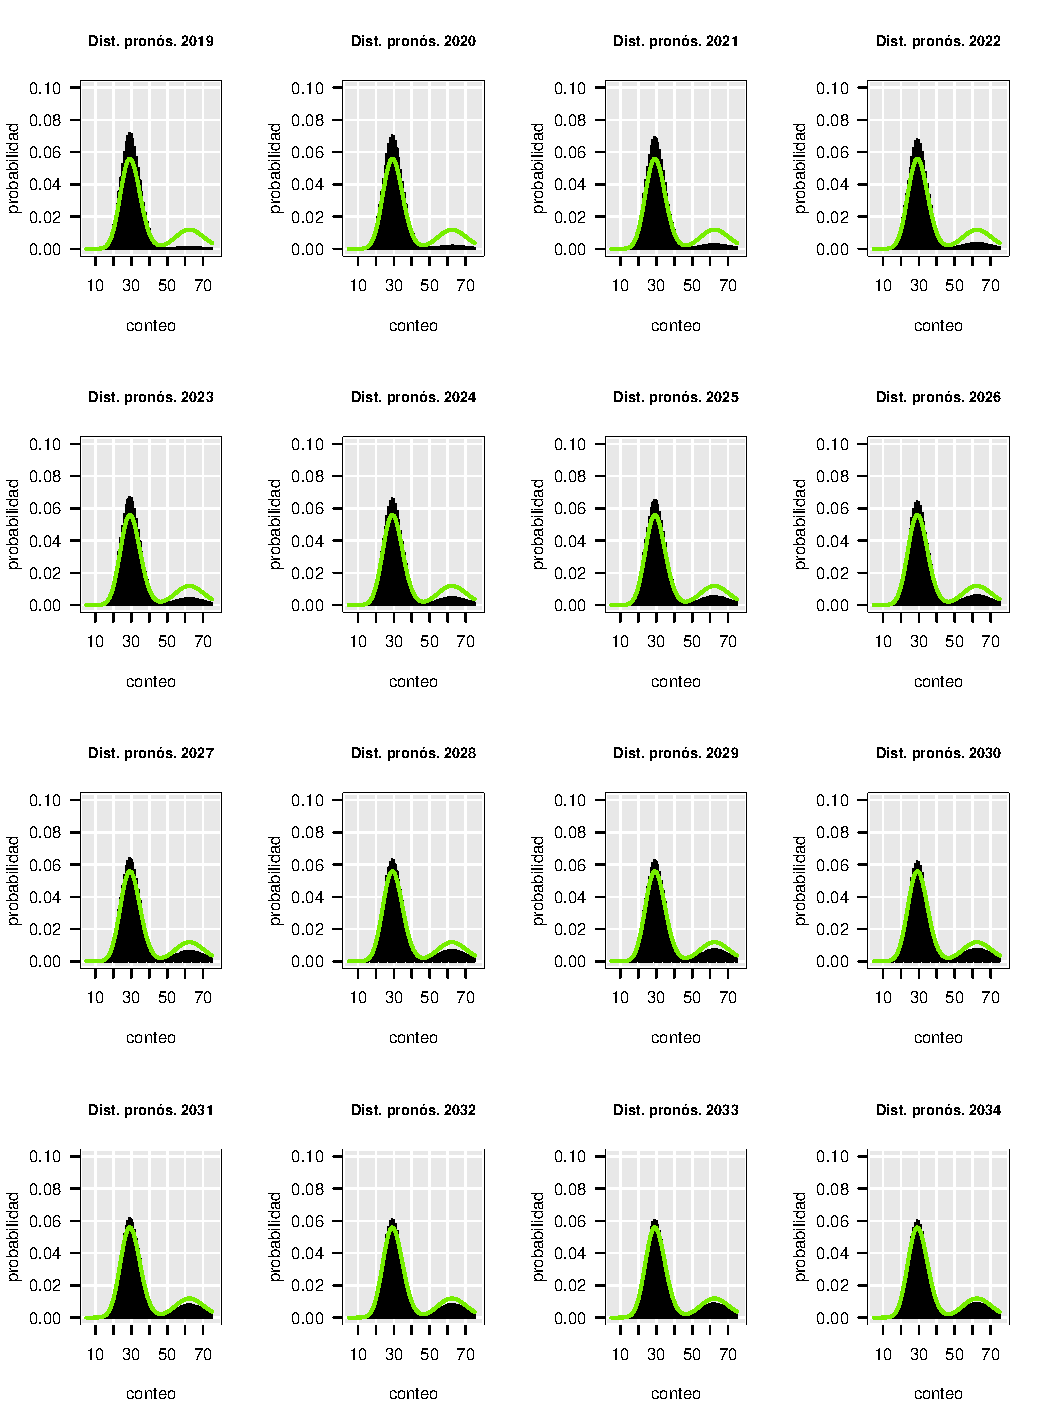
\includegraphics[width=\maxwidth]{figure/unnamed-chunk-19-1} \caption[Pronostico de la distribución para los años 2019 a 2034]{Pronostico de la distribución para los años 2019 a 2034.}\label{fig:unnamed-chunk-19}
\end{figure}


\end{knitrout}

Se realiza la predicción de los estados más probables para los proximos 16 años, tambien podemos pronosticar la distribución para estos mismos años. Como se observa en la figura 8 a medida que el horizonte de pronóstico $h$ aumenta, la distribución de pronóstico converge a la distribución marginal del HMM estacionario. En la tabla 7, se observa que el prónstico de los estados, para los próximos 16 años es el 1, es decir que se espera una tasa de homidios por cada 100.000 habitantes cercana a 29, la cual sigue siendo alta ya que según datos de la ONUDD (Oficina de Naciones Unidas contra la Droga y el Delito), en sur America la tasa se situa en 20/100.000 homicidios, lo que indica quee la tasa de homicidios en  Colombia está por encima de la región. Además según estadísticas de la ONUDD, Colombia se situa como uno de los países más violentos del mundo ubicandose en el top 20, las cifras de la fiscalia indican que despues de haber disminuido la tasa de homidios en los últimos años, a partir del 2018 hubo un incremento del $3.25 \%$, de este delito siendo caso críticos las ciudades de Medellín, bajo Cauca y Tumaco, mientras la capital sigue con tendencia a la baja.

% latex table generated in R 3.6.0 by xtable 1.8-4 package
% Sun Jul 14 00:13:45 2019
\begin{table}[ht]
\centering
\begin{tabular}{rrrr}
  \hline
Año & Estado 1 & Estado 2 & Estado \\ 
  \hline
 2019 & 0.9802 & 0.0198 &     1 \\ 
   2020 & 0.9621 & 0.0379 &     1 \\ 
   2021 & 0.9456 & 0.0544 &     1 \\ 
   2022 & 0.9304 & 0.0696 &     1 \\ 
   2023 & 0.9164 & 0.0836 &     1 \\ 
   2024 & 0.9037 & 0.0963 &     1 \\ 
   2025 & 0.8920 & 0.1080 &     1 \\ 
   2026 & 0.8813 & 0.1187 &     1 \\ 
   2027 & 0.8714 & 0.1286 &     1 \\ 
   2028 & 0.8624 & 0.1376 &     1 \\ 
   2029 & 0.8542 & 0.1458 &     1 \\ 
   2030 & 0.8467 & 0.1533 &     1 \\ 
   2031 & 0.8397 & 0.1603 &     1 \\ 
   2032 & 0.8334 & 0.1666 &     1 \\ 
   2033 & 0.8276 & 0.1724 &     1 \\ 
   2034 & 0.8223 & 0.1777 &     1 \\ 
   \hline
\end{tabular}
\caption{Predicción para las probabilidades de los estados hasta un rezago h = 16.} 
\end{table}


En el siguiente apartado se muestran las estimaciones bayesianas realizadas a la serie homicidios

%http://www.scielo.br/pdf/csc/v17n12/06.pdf

\clearpage

\subsubsection*{Estimación Bayesiana del PHMM}





Primero se ajustaron cuatro modelos, con la función `Bayeshmmcts::bayes.PHMM`, para 2, 3, 4 y 5 estados, después, se estimo la $\log$ - verosimilitud marginal, utilizando muestreo por puente como alternativa a las propuesta hecha por Newton y Raftery (1994) que sugiere utilizar la verosimilitud integrada, para hallar el estimador de la media armónica de los valores de la verosimilitud de una muestra obtenida desde la distribución posterior. Pero como se vio en la sección (4), aunque el estimador es consitente tiene un gran problema varianza infinita. Mientras que el estimador del muestreador por puente, no presenta ese problema además de su facil implementación, pues esta metodología se puede ejecutar con la función `bridge sampler` del paquete bridgesampling, del autor Gronau. El paquete \textbf{bridgesampling}, permite además calcular el error de la estimación para la verosimilitud marginal, obtendido via muestreo por puente que en el caso del modelo con dos estados, el error es de $0.478 \%$. 

Un factor de Bayes es la relación entre la probabilidad de una hipótesis particular y la probabilidad de otra. Puede interpretarse como una medida de la fuerza de la evidencia en favor de una teoría entre dos teorías en competencia. Esto se debe a que el factor de Bayes nos permite evaluar los datos a favor de una hipótesis nula y utilzar información externa para hacerlo. Nos dice cuál es el peso de la evidencia a favor de una hipótesis dada.

Cuando estamos comparando dos hipótesis, $H_0$ (la hipótesis nula) y $H_1$ (la hipótesis alternativa) y , el factor de Bayes a menudo se escribe como $B_{01}$. Se puede definir matemáticamente como

$$B_{01} = \frac{\text{verosimilitud de los datos dado $H_0$}}{\text{verosimilitud de los datos dado $H_1$}} = \frac{P(D | H_0)}{P(D | H_1)}$$

El factor de Bayes puede es un número positivo, y una de las interpretaciones más comunes es esta: propuesta por primera vez por Harold Jeffereys(1961) y modificada ligeramente por Lee y Wagenmakers en 2013:

% latex table generated in R 3.6.0 by xtable 1.8-4 package
% Sun Jul 14 00:13:45 2019
\begin{table}[ht]
\centering
\begin{tabular}{ll}
  \hline
B01 & Desición \\ 
  \hline
$>$100 & Evidencia extrema para H0 \\ 
  30 - 100 & Evidencia muy fuerte para H0 \\ 
  10 - 30 & Evidencia fuerte para H0 \\ 
  3 - 10 & Evidencia moderada para H0 \\ 
  1 - 3 & Evidencia apenas mencionable para H0 \\ 
  1 & No hay evidencia \\ 
  1/3 - 1 & Evidencia apenas mencionable para H1 \\ 
  1/10 - 1/3 & Evidencia moderada para H1 \\ 
  1/30 - 1/3 & Evidencia fuerte para H1 \\ 
  1/100 - 1/30 & Evidencia muy fuerte para H1 \\ 
  $<$ 1/100 & Evidencia extrema para H1 \\ 
   \hline
\end{tabular}
\caption{Interpretación del factor de Bayes, Lee y Wagenmakers (2013).} 
\end{table}


Ahora utilizamos el factor de bayes para contrastar los modelos con m-estados de a parejas, y seleccionar el más adecuado, en la siguiente tabla ilustra el contraste de hipótesis, donde las filas indican $P(D | H_0)$ y las columnas $P(D | H_1)$. Por ejemplo en el contraste de hipótesis entre el modelo de 3 estados vs el modelo de 4 estados, el valor obtenido fue $B_{01} = 766.05$, lo que indica evidencia extrema para $H_0$, es decir el modelo de 3 estados es más apropiado que el de 4 estados.

% latex table generated in R 3.6.0 by xtable 1.8-4 package
% Sun Jul 14 00:13:45 2019
\begin{table}[ht]
\centering
\begin{tabular}{rrrrr}
  \hline
 & mod 2 Estados & mod 3 Estados & mod 4 Estados & mod 5 Estados \\ 
  \hline
mod 2 Estados &  & 3.36 & 2545.85 & 390147608.00 \\ 
  mod 3 Estados &  &  & 766.05 & 125542040.00 \\ 
  mod 4 Estados &  &  &  & 128023.00 \\ 
   \hline
\end{tabular}
\caption{Comparación resultados Factor de Bayes para los PHMM.} 
\end{table}




De la tabla 9, se concluye que el modelo apropiado es el de orden 2, lo cual coincide con el BIC. Se corrieron 5.000 iteraciones con 3 cadenas y las primeras 2.500 iteraciones de calentamiento adelgazando la cadena cada 3 iteraciones; con tasa de aceptación para la función objetivo en el metropolis de 0.99. A continuación mostramos las estimaciones bayesianas de la matriz de transición, y la media de los estados dependientes:

% latex table generated in R 3.6.0 by xtable 1.8-4 package
% Sun Jul 14 00:13:46 2019
\begin{table}[ht]
\centering
\begin{tabular}{rrrrrrrrrrr}
  \hline
 & Media & Err.Sta & Desv & 2.5\% & 25\% & 50\% & 75\% & 97.5\% & n\_eff & Rhat \\ 
  \hline
$a_{11}$ & 0.953 & 0.001 & 0.032 & 0.873 & 0.935 & 0.961 & 0.977 & 0.994 & 2491.677 & 1.000 \\ 
  $a_{12}$ & 0.047 & 0.001 & 0.032 & 0.006 & 0.023 & 0.039 & 0.065 & 0.127 & 2491.677 & 1.000 \\ 
  $a_{21}$ & 0.099 & 0.001 & 0.065 & 0.014 & 0.051 & 0.084 & 0.133 & 0.257 & 2417.781 & 1.000 \\ 
  $a_{22}$ & 0.901 & 0.001 & 0.065 & 0.743 & 0.867 & 0.916 & 0.949 & 0.986 & 2417.781 & 1.000 \\ 
  $\lambda_1$ & 29.715 & 0.018 & 0.871 & 28.097 & 29.111 & 29.684 & 30.299 & 31.460 & 2456.451 & 1.001 \\ 
  $\lambda_2$ & 62.849 & 0.039 & 1.961 & 59.068 & 61.491 & 62.811 & 64.184 & 66.735 & 2560.484 & 1.000 \\ 
  lp & -210.558 & 0.030 & 1.426 & -214.125 & -211.268 & -210.260 & -209.512 & -208.739 & 2200.204 & 1.002 \\ 
   \hline
\end{tabular}
\caption{Estimación bayesiana de los parámetros para un PHMM.} 
\end{table}


Para cada parámetro estimado a partir de las muestras obtenidas por MCMC se calculo, la media de las tres cadenas fusionadas. También se calculo el error estándar es aquel el error debido a la estimación de la media poblacional a partir de las medias muestrales. La desviación estándar para este caso indica una dispersión muy pequeña tanto en la estimación de la tpm como del vector de medias de los estados dependientes. Se calculan los intervalos de credibiliddad al $95 \%$, y la mediana de las estimaciones que distan muy poco de la media, lo que indica que en el proceso de muestreo no hubo valores atípicos o extremos.
Stan define el logaritmo de la función de densidad de probabilidad de una distribución posterior hasta una constante aditiva desconocida. Usando a lp para representar las realizaciones de este $\log$ kernel en cada iteración ($lp$ se trata como una incógnita en el resumen y el cálculo de la división $\hat{R}$ y el tamaño de muestra efectivo).

% latex table generated in R 3.6.0 by xtable 1.8-4 package
% Sun Jul 14 00:13:47 2019
\begin{table}[ht]
\centering
\begin{tabular}{rrrrrrrrrrrrrrrrrrrr}
  \hline
  \hline
1 & 1 & 1 & 1 & 1 & 1 & 1 & 1 & 1 & 1 & 1 & 1 & 1 & 1 & 1 & 1 & 1 & 1 & 1 & 1 \\ 
  1 & 1 & 1 & 1 & 1 & 1 & 2 & 2 & 2 & 2 & 2 & 2 & 2 & 2 & 2 & 2 & 2 & 2 & 2 & 2 \\ 
  2 & 2 & 2 & 2 & 2 & 1 & 1 & 1 & 1 & 1 & 1 & 1 & 1 & 1 & 1 & 1 & 1 & 1 & 1 &  \\ 
   \hline
\end{tabular}
\caption{Resultados de la decodificación global bayesiana para el PHMM orden 2, con el algoritmo Viterbi.} 
\end{table}


\begin{knitrout}
\definecolor{shadecolor}{rgb}{0.91, 0.91, 0.91}\color{fgcolor}\begin{figure}
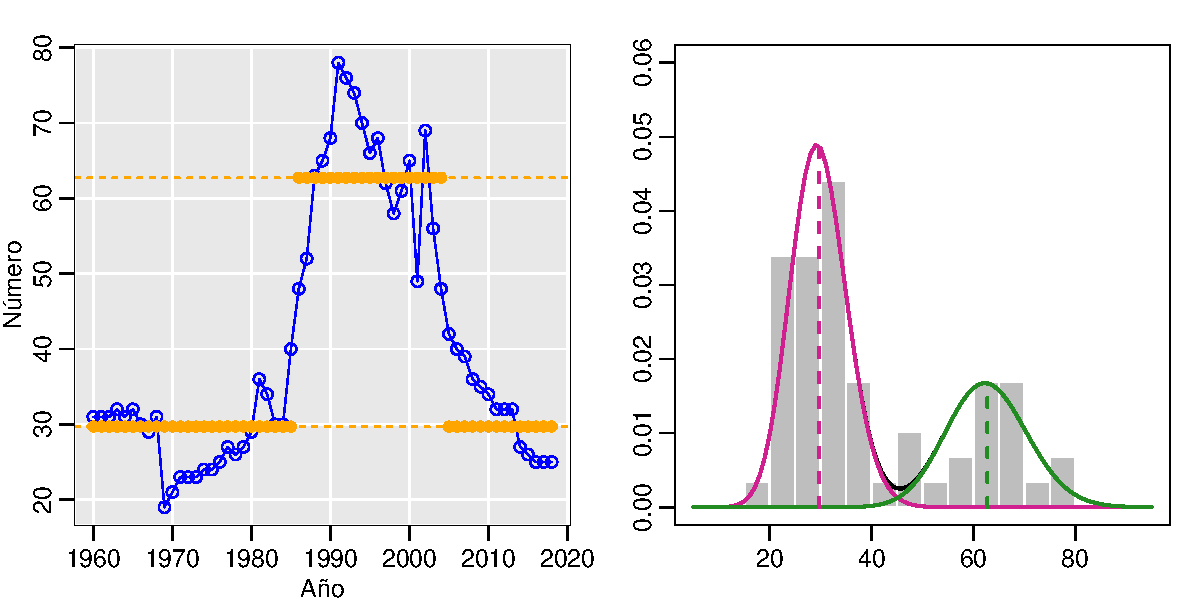
\includegraphics[width=\maxwidth]{figure/unnamed-chunk-28-1} \caption[Algoritmo Viterbi aplicado a un PHMM de dos estados]{Algoritmo Viterbi aplicado a un PHMM de dos estados.}\label{fig:unnamed-chunk-28}
\end{figure}


\end{knitrout}

Hay dos estadísticas de diagnóstico realmente importantes ocultas en este resumen:

\begin{itemize}
  \item $n\_eff$: el tamaño efectivo de la muestra.
  \item $Rhat$: la ``estadística de reducción de escala de potencial de Gelman y Rubin".
\end{itemize}

$n\_eff$ mide el tamaño de muestra efectivo de ese parámetro en particular. Recuerde que cada iteración de la HMC se basa en el valor del parámetro en la iteración anterior. Sin embargo, idealmente, si el algoritmo funciona correctamente, el parámetro elegido en la siguiente iteración será independiente de ese valor de parámetro inicial (esto es lo que el "adelgazamiento" debe lograr en otros MCMC, aunque también puede hacerlo usando HMC). Sin embargo, si no está realizando un trabajo muy eficiente al muestrear el espacio de parámetros, es más probable que los valores de los parámetros en una iteración dada estén cerca de los valores de los parámetros en la última iteración. Esto significa que estos parámetros no son realmente independientes por ejemplo se tiene 1000 muestras obtenidas de la distribución posterior, es posible que no se tenga 1000 muestras independientes del parámetro, sino un número menor de muestras verdaderamente ``independientes".
\\
Entonces, $n\_eff$ es la suma de las iteraciones de muestreo efectivamente independientes en todas las cadenas. En este caso, tenemos 3 cadenas, con 5000 iteraciones, la mitad de las cuales son de calentamiento, lo que significa que muestreamos 2500 iteraciones en cada cadena, por lo que el máximo $n\_eff$ posible en este caso es 7500.
\\
La mayoría de nuestros parámetros tienen un $n\_eff$ bastante alto, aunque vemos que algunos son un poco más bajos. ¿Cómo sabemos si un $n\_eff$ como 2500 (de 7500 posibles) es demasiado bajo?. El estadístico Rhat nos ayuda a saber si estos parámetros están tan mal muestreados que tenemos un problema. Más o menos Rhat le dice si cada una de las cadenas ha alcanzado o no una distribución posterior estable, a pesar de comenzar con diferentes valores iniciales. Gelman recomienda que Rhat para cada parámetro sea inferior a 1.1.
\\
En la parte izquierda de la figura 8 y en la tabla 11, se muestra la decodificación global de la secuencia de estados más probables, para la serie homicidios en Colombia. Al igual que otros algoritmos de programación dinámica, Viterbi funciona de forma recursiva; encontrando el estado más probable al tomar el máximo sobre todas las posibles secuencias de estados anteriores. Dada la secuencia de observaciones sobre homicidios en Colombia y los modelos clásico con el bayesiano de orden dos, dan exactamente los mismos resultados. Mientras que la parte derecha de la figura 8 muestra las distribuciones marginales, utilizadas para hacer el prónostico de las distribuciones para un rezago $h$ dado.

% latex table generated in R 3.6.0 by xtable 1.8-4 package
% Sun Jul 14 00:13:47 2019
\begin{table}[ht]
\centering
\begin{tabular}{rrrr}
  \hline
 & Estado 1 & Estado 2 & Estado \\ 
  \hline
2019 & 0.9533 & 0.0467 &     1 \\ 
  2020 & 0.9134 & 0.0866 &     1 \\ 
  2021 & 0.8793 & 0.1207 &     1 \\ 
  2022 & 0.8502 & 0.1498 &     1 \\ 
  2023 & 0.8253 & 0.1747 &     1 \\ 
  2024 & 0.8040 & 0.1960 &     1 \\ 
  2025 & 0.7859 & 0.2141 &     1 \\ 
  2026 & 0.7703 & 0.2297 &     1 \\ 
  2027 & 0.7571 & 0.2429 &     1 \\ 
  2028 & 0.7457 & 0.2543 &     1 \\ 
  2029 & 0.7361 & 0.2639 &     1 \\ 
  2030 & 0.7278 & 0.2722 &     1 \\ 
  2031 & 0.7207 & 0.2793 &     1 \\ 
  2032 & 0.7147 & 0.2853 &     1 \\ 
  2033 & 0.7095 & 0.2905 &     1 \\ 
  2034 & 0.7051 & 0.2949 &     1 \\ 
   \hline
\end{tabular}
\caption{Predicción bayesiana para las probabilidades de los estados hasta un rezago h = 16.} 
\end{table}


La tabla 12 muestra, las probabilidades correspondientes a la predicción de los rezagos para un $h \in \mathbb{N}$. El error de la predicción aumenta a medida que crece el horizonte en el tiempo, por ejemplo para los dos proximos años 2019 y 2020, la probabilidad de estar en el estado 1 es mayor al $90 \%$ mientrass que para los años 2033 y 2034, la probabilidad de estar en el estado 1 se reduce a un $70 \%$, sin embargo en los proximos 16 años se espera que la tasa de homicidios este alrededor 30 muertes por cada 100.000 habitantes.

\subsubsection*{Diagnosticos de la cadena}

En esta sección se verificara el diagnostico de convergencia de las cadenas utilizadas en la extracción de las muestras. Para los métodos MCMC ajustados con \textbf{Stan}, ya sean Hamiltonian Monte (HMC) o No-U-Turn-Sampler (NUTS), el paquete \emph{bayesplot} y \emph{coda}, cuenta con una serie de herrmientas gráficas y purebas diagnosticas para después del ajuste de modelos bayesianos. En la figura No se muestra los histogramas univariados y diagramas de dispersión bivariados para los parámetros de la matriz de transición de probabilidad y para el vector de medias de los estados dependientes, especialmente útil para identificar la colinealidad entre variables (que se manifiesta como gráficos bivariados estrechos), así como la presencia de no-identificabilidad multiplicativa (formas tipo plátano).

En sentido estricto, la no identificabilidad significa que dos valores de los parámetros dan como resultado la misma distribución de probabilidad de los datos observados. Algunas veces también se usa para cubrir situaciones en las que no hay un máximo local único de la densidad posterior, ya sea porque hay múltiples máximos separados o porque hay una meseta donde un conjunto de puntos tiene la misma densidad posterior (estos pueden o pueden No ser identificable en sentido estricto).

En la figura 9 se observa que no parece haber problemas con la identificabilidad, es decir que no existen problemas que señalan divergencias, lo único que se observa es colinealidad entre los parámetros de las filas de la matriz de transición, sin embargo recordemos por definición que la suma de las filas de la tpm suman 1, por lo tanto están de por si correlacionadas. Por lo tanto como el modelo es identificable, no estamos asegurando que las inferencias no están sesgadas.

\vspace{5mm} %5mm vertical space

El gráfico de traza, muestra por cada una de las iteraciones los valores muestreados correspondiente a una o más cadenas de Markov, separado por parámetro. Las cadenas proporcionan una forma visual para inspeccionar el comportamiento de muestreo y evaluar la mezcla a través de las cadenas y la convergencia, como vemos se comportana bastante bien, pues hay un mínimo de muestras divergentes.

\begin{knitrout}
\definecolor{shadecolor}{rgb}{0.91, 0.91, 0.91}\color{fgcolor}\begin{figure}[h]
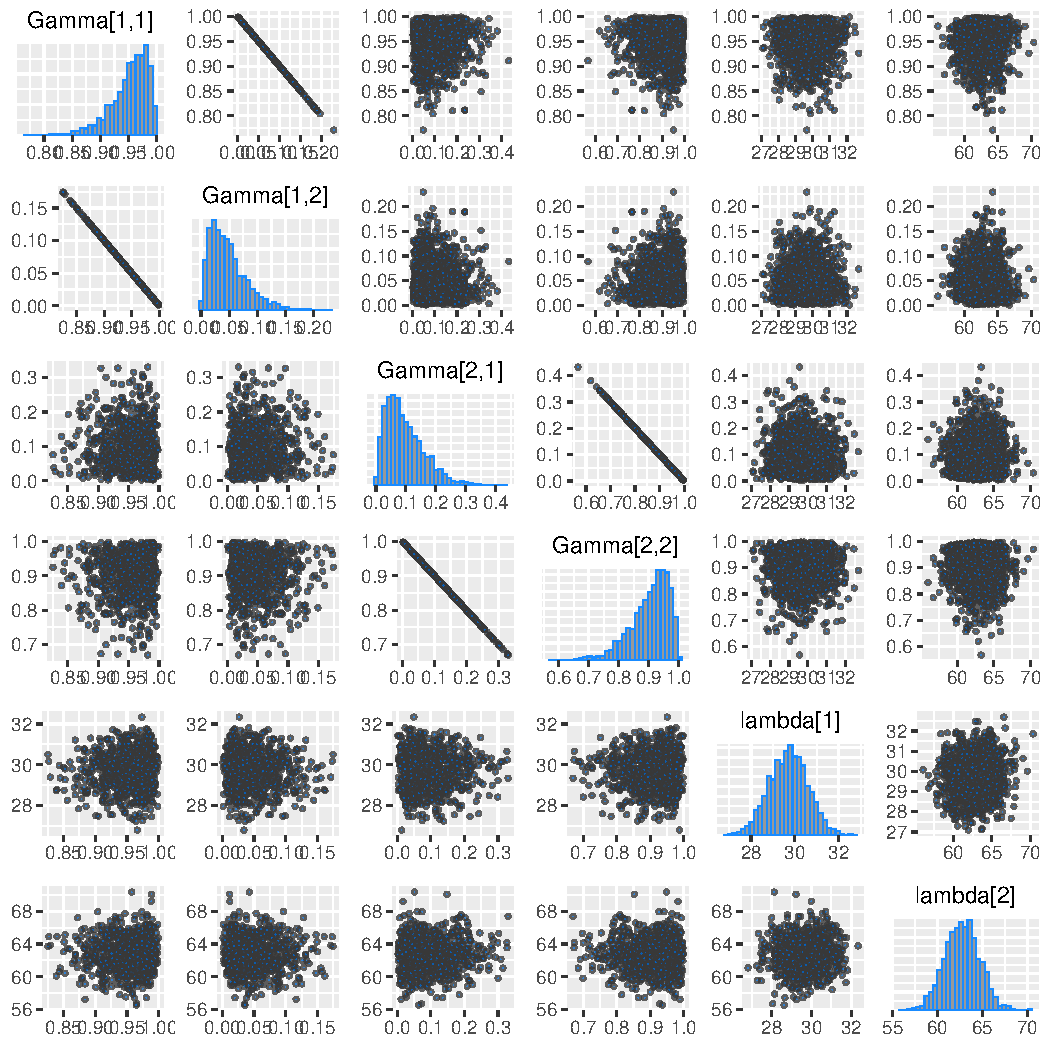
\includegraphics[width=\maxwidth]{figure/unnamed-chunk-30-1} \caption[Gráfico de trazas de las cadenas, para cada iteración y por cadena]{Gráfico de trazas de las cadenas, para cada iteración y por cadena.}\label{fig:unnamed-chunk-30}
\end{figure}


\end{knitrout}
                              
Los intervalos de credibilidad, para los parámetros calculados a partir de las muestras posteriores con todas las cadenas fusionadas. Los resultados índican valores consistentes en las estimaciones de los parámetros, pues la longitud del intervalo es bastante pequeña como se mostrara más adelante.

\begin{knitrout}
\definecolor{shadecolor}{rgb}{0.91, 0.91, 0.91}\color{fgcolor}\begin{figure}
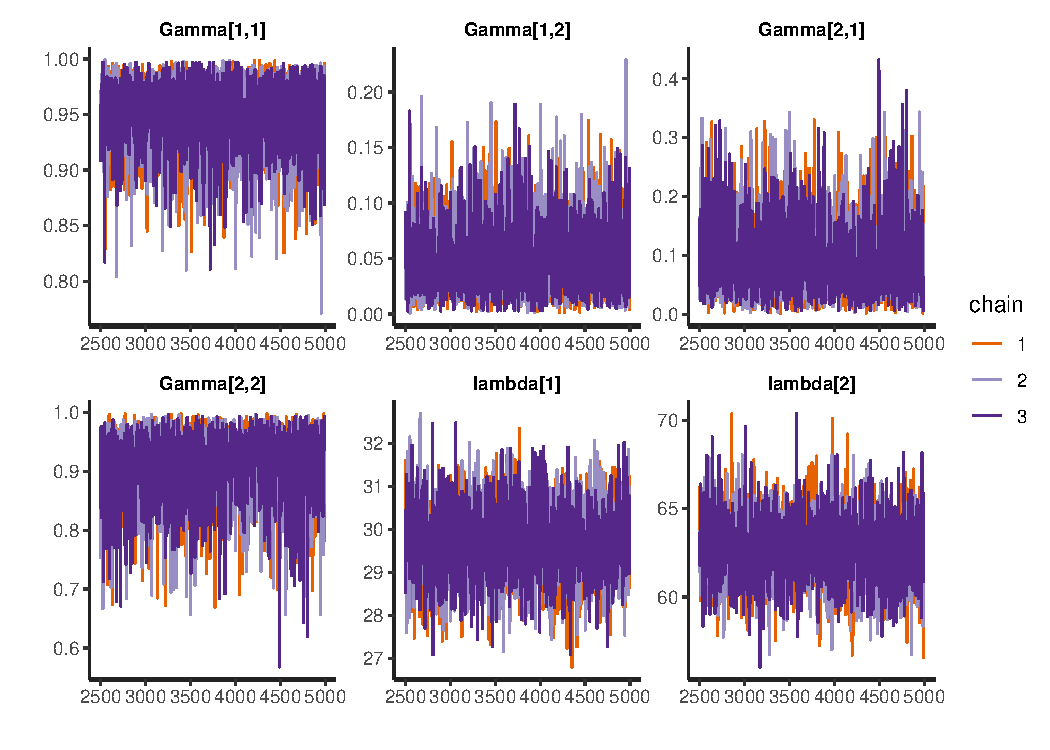
\includegraphics[width=\maxwidth]{figure/unnamed-chunk-31-1} \caption[Intervalos de crédibilidad al 0.95 PHMM]{Intervalos de crédibilidad al 0.95 PHMM.}\label{fig:unnamed-chunk-31}
\end{figure}


\end{knitrout}

\vspace{5mm} %5mm vertical space

\begin{knitrout}
\definecolor{shadecolor}{rgb}{0.91, 0.91, 0.91}\color{fgcolor}\begin{figure}
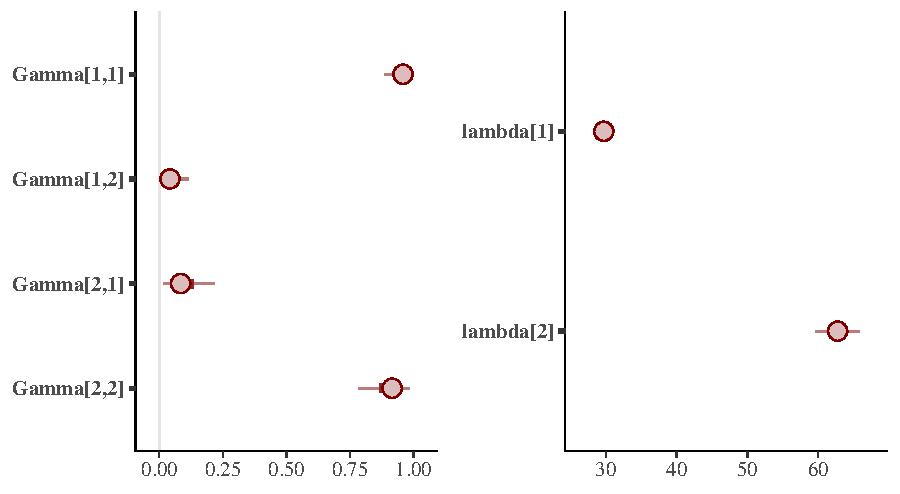
\includegraphics[width=\maxwidth]{figure/unnamed-chunk-32-1} \caption[Gráfico de dispersión para las muestras MCMC]{Gráfico de dispersión para las muestras MCMC.}\label{fig:unnamed-chunk-32}
\end{figure}


\end{knitrout}

La prueba de convergencia utiliza la estadística de Cramer-von-Mises para probar la hipótesis nula de que los valores muestreados provienen de una distribución estacionaria. La prueba se aplica sucesivamente, primero a toda la cadena, luego, después de descartar el primer $10 \%$, $20 \%$, ... de la cadena hasta que se acepte la hipótesis nula, o se haya descartado el $50 \%$ de la cadena. El último resultado constituye un \emph{fallo} de la prueba de estacionariedad e indica que se necesita una ejecución MCMC más larga. Si se pasa la prueba de estacionariedad, se informa el número de iteraciones a mantener y el número a descartar.

La prueba de medio ancho calcula un intervalo de confianza del $95 \%$ para la media, utilizando la parte de la cadena que pasó la prueba de estacionariedad. La mitad del ancho de este intervalo se compara con la estimación de la media. Si la relación entre la mitad del ancho y la media es menor que \emph{eps}, se pasa la prueba de la mitad del ancho. De lo contrario, la longitud de la muestra no se considera lo suficientemente larga como para estimar la media con suficiente precisión.

% latex table generated in R 3.6.0 by xtable 1.8-4 package
% Sun Jul 14 00:14:14 2019
\begin{table}[ht]
\centering
\begin{tabular}{rlrlrr}
  \hline
 & P. Estacionariedad & Valor p & Prueba & Media & Medio.Ancho \\ 
  \hline
$a_{11}$ & páso & 0.396 & páso & 0.953 & 0.001 \\ 
  $a_{21}$ & páso & 0.978 & páso & 0.099 & 0.002 \\ 
  $a_{12}$ & páso & 0.396 & páso & 0.047 & 0.001 \\ 
  $a_{22}$ & páso & 0.978 & páso & 0.901 & 0.002 \\ 
  $\lambda_1$ & páso & 0.569 & páso & 29.701 & 0.034 \\ 
  $\lambda_2$ & páso & 0.862 & páso & 62.742 & 0.079 \\ 
  lp & páso & 0.440 & páso & -210.525 & 0.062 \\ 
   \hline
\end{tabular}
\caption{Prueba de estacionariedad, usando el estadístico de Cramer-von-Mises para la convergencia de la cadena y prueba de medio ancho para la media calculando el intervalo de confianza al 0.95.} 
\end{table}


\clearpage

\subsubsection{Comparación PHMM clásico vs Bayesiano}

La inferencia para los parámetros bajo el enfoque clásico se realizo utilizando bootstrap (Zucchini (2016)). El método bootstrap es una técnicas de remuestreo diseñadas para aproximar la función de distribución de probabilidad de los datos mediante una función empírica de una muestra finita. El método bootstrap se puede usar para estimar los intervalos de confianza directamente. Se utilizo el ``método de percentil" (Efron y Tibshirani, 1993) para estimar los intervalos, se generaron 250 muestras independientes a partir del PHMM de orden 2 de longitud 59 igual a la serie homicidios en Colombia. Los valores iniciales usados fueron los estimados por PHMM de 2 estados con el fin de evitar inestabilidad numérica o problemas de convergencia. Los intervalos de credibilidad fueron calculados a partir de las distribuciones aposteriori de los parámetros de las muestras generadas por MCMC. El nivel y la probabilidad de los intervalos de confianza y credibilidad, respectivamente, se fijaron en 0.95.



% latex table generated in R 3.6.0 by xtable 1.8-4 package
% Sun Jul 14 00:14:15 2019
\begin{table}[ht]
\centering
\begin{tabular}{lrrrrrrrr}
  \toprule
   & \multicolumn{4}{c}{\textbf{Intervalos de Credibilidad}} & \multicolumn{4}{c}{\textbf{Intervalos de Confianza}}\\
 \cmidrule(lr){2-5}\cmidrule(lr){6-9}
 \textbf{Parámetros} & \textbf{Media} & \textbf{2.5} & \textbf{97.5} & \textbf{Ancho} & \textbf{Media} & \textbf{2.5} & \textbf{97.5} & \textbf{Ancho}\\
 \midrule
$a_{11}$ & 0.953 & 0.873 & 0.994 & 0.120 & 0.980 & 0.844 & 1.000 & 0.156 \\ 
  $a_{21}$ & 0.099 & 0.014 & 0.257 & 0.244 & 0.064 & 0.015 & 1.000 & 0.985 \\ 
  $a_{12}$ & 0.047 & 0.006 & 0.127 & 0.120 & 0.020 & 0.000 & 0.156 & 0.156 \\ 
  $a_{22}$ & 0.901 & 0.743 & 0.986 & 0.244 & 0.936 & 0.000 & 0.985 & 0.985 \\ 
  $\lambda_1$ & 29.715 & 28.097 & 31.460 & 3.363 & 29.716 & 27.689 & 31.648 & 3.959 \\ 
  $\lambda_2$ & 62.849 & 59.068 & 66.735 & 7.667 & 62.813 & 30.140 & 68.497 & 38.357 \\ 
   \bottomrule
\end{tabular}
\caption{Intervalos de Credibilidad y Confianza para el PHMM de orden 2.} 
\end{table}


Al calcular los intervalos de confianza y de credibilidad, es importante determinar cuál de estos métodos son más eficaces. Para determinar el comportamiento de los intervalos propuestos, usualmente se utiliza, la longitud del intervalo, su probabilidad de cobertura el valor esperado y la varianza de su longitud. Un buen método debe tener valores pequeños en la longitud del intervalo, en su valor esperado y en la varianza de su longitud; con probabilidades de cobertura cercanas a los niveles de confianza nominal.
\\
La longitud del intervalo, que indica su precisión, se muestran en la tabla 14, junto con la media de las estimaciones en el caso Bayesiano y el estimador de máxima verosimilitud para el caso clásico. Tanto para los parámetros de la matriz de transición como para el vector de medias de los estados dependientes, los intervalos de credibilidad indican una longitud menor es decir mayor precisión. Por lo que en este caso podríamos decir que las estimaciones bayesianas son más precisas y por lo tanto el enfoque bayesiano parece ser el más apropiado.  

Finalmente, aunque el intervalo de credibilidad difiere de la interpretación del intervalo de confianza, permite juzgar la incertidumbre estadística para la tasa de homicidios suponiendo el PHMM subyacente válido. Mientras el intervalo de confianza indica que el $95 \%$ de los intervalos de confianza generado por un mismo procedimiento incluyen el verdadero valor del parámetro. El intervalo de credibilidad representa con una probabilidad del $95 \%$ que el intervalo incluya el verdadero valor de la población objetivo siempre que el modelo adoptado sea válido. 

\clearpage

\subsection{Modelo Poisson Cero inflado - Oculto de Markov}



En esta sección utilizaremos, los datos de incendios forestales en Colombia, desde enero del 2001 hasta diciembre del 2016. La variable de interés es el número de grandes incendios forestales (GIF), que son aquellos incendios que superan las 500 hectáreas forestales afectadas. La periodicidad de los datos es mensual con un total 180 observaciones, en la Tabla 11 se muestran los primeros 12 registros, mientras que la Tabla 12 indica la frecuencia. Allí observamos que hay una alta proporción de ceros en los datos, pues de las 180 observaciones 124 son cero, es decir el $68.9 \%$ de los registros. Por otra parte el número máximo de GIF ocurridos en un mes en Colombia fue 23 en febrero del 2017, lo cual es preocupante; pues aunque los incendios forestales naturales han ocurrido desde siempre como un elemento normal en el funcionamiento de los ecosistemas. El fuego ha permitido la regeneración de diversos ecosistemas y la producción de una serie de hábitats en los que distintos organismos pueden prosperar. No obstante notemos que el promedio de GIF se ubico en $1.3 \pm 3.5$ incendio por mes, haciendo que la enorme proliferación de los incendios a causa de la actividad humana en estas últimas décadas sobrepasa la capacidad de recuperación natural.

\begin{knitrout}
\definecolor{shadecolor}{rgb}{0.91, 0.91, 0.91}\color{fgcolor}\begin{figure}[h]
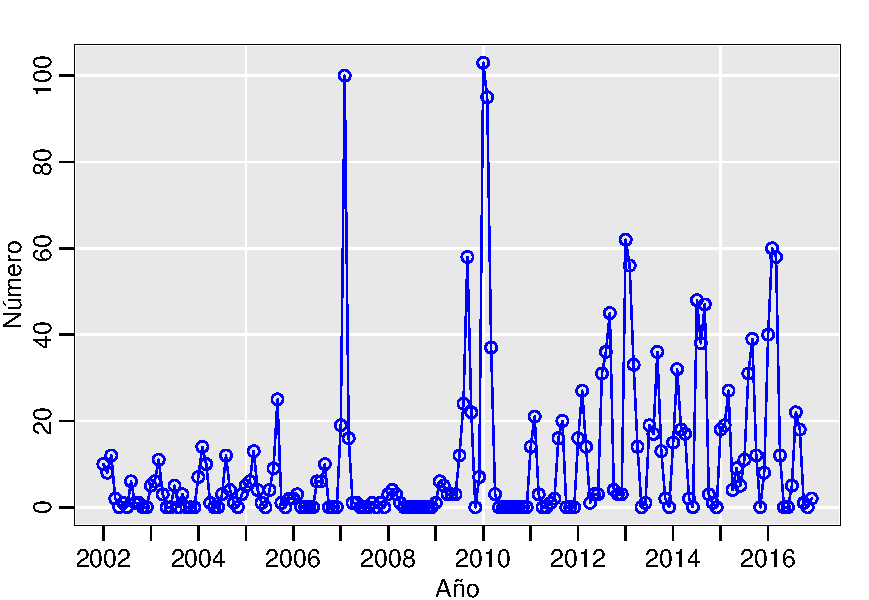
\includegraphics[width=\maxwidth]{figure/unnamed-chunk-37-1} \caption[Serie de tiempo Grandes Incendios Forestales en Colombia desde el año 2002 hasta el año 2016]{Serie de tiempo Grandes Incendios Forestales en Colombia desde el año 2002 hasta el año 2016.}\label{fig:unnamed-chunk-37}
\end{figure}


\end{knitrout}

En la figura 12, se observa dos picos altos en el 2007 y el 2010. Después del año 2011 la cero inflación disminuye considerablemente y el número de incendios en gran parte de los meses parece estar por encima de 5, este fenómeno se presenta de manera recurrente en gran parte del país, en especial durante los periodos secos prolongados, durante los cuales los ecosistemas tropicales húmedos y muy húmedos pierden parte de los contenidos de humedad superficial e interior, incrementando sus niveles de susceptibilidad y amenaza hacia la combustión de la biomasa vegetal que los compone. En la tabla 2 se encuentran todos los datos de GIF en Colombia.
\\
Para determinar si existe correlación entre los GIF de cada mes, se calcula la función de autocorrelación muestral, la figura 14 indica no solo la existencia de la dependencia serial sino una estructura estacional.

\begin{knitrout}
\definecolor{shadecolor}{rgb}{0.91, 0.91, 0.91}\color{fgcolor}\begin{figure}
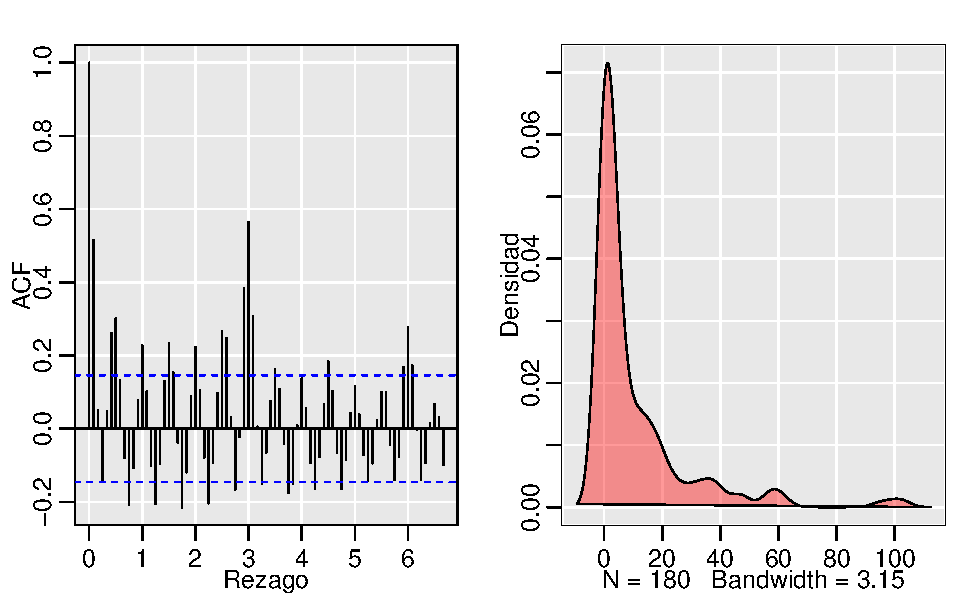
\includegraphics[width=\maxwidth]{figure/unnamed-chunk-38-1} \caption[Función de autocorrelación muetral, y kernel de densidad para la serie Grandes Incendios Forestales en Colombia (2002-2016)]{Función de autocorrelación muetral, y kernel de densidad para la serie Grandes Incendios Forestales en Colombia (2002-2016).}\label{fig:unnamed-chunk-38}
\end{figure}


\end{knitrout}

Como se vio en la figura 14, existe dependencia serial entre los GIF mensuales ocurridos de Colombia, además parece haber una estructura estacional entre los meses donde ocurrieron estos incendios. Además la densidad estimada por kernel, muestra diferentes picos concentrandose los valores principalmente en cero.

\subsubsection{Ajuste del ZIP-HMM}

Se ajustaron seis modelos ZIP-HMM con 2 a 6 estados, utilizando el paquete \textbf{ziphsmm} creado por Zekun Xu, que permite ajusar modelos Poisson cero Inflados - Ocultos de Markov, estimando los parámetros vía directa minimización de la función log verosimilitud usando el algoritmo descenso del gradiente. Se utilizo el método de Nelder-Mead con 1.000 iteraciones con el fin de evitar máximos locales. En la tabla 15 se registro para cada modelo el número de parámetros estimados, la log-verosimilitud el criterio de información de Akaike (AIC) y el criterio de información bayesiano (BIC).
\\
Para seleccionar el modelo más apropiado, se debe escoger el valor que minimiza el AIC, en este caso es el ZIP HMM de 6 estados con un Akaike de 1101, sin embargo el criterio de Schwarz con un valor de 1176 indica que el modelo más apropiado es el de orden 4, esta es una dicotomia que puede presentarse en ocasiones. Sin embargo decidimos escoger como criterio el BIC para la selección del modelo por dos razones principalmente. Primero porque el BIC generalmente penaliza parámetros libres con más fuerza de lo que lo hace el Akaike, y segundo porque para calcular el modelo de 6 estados es necesario calcular el doble de parámetros con respecto al de 4, haciendolo más costoso computacionalmente, pues con cada estado adicional el número de parámetros a estimar crece de manera sustancial.



% latex table generated in R 3.6.0 by xtable 1.8-4 package
% Sun Jul 14 00:14:16 2019
\begin{table}[ht]
\centering
\begin{tabular}{rlrrrr}
  \hline
 & Modelo & p & logL & AIC & BIC \\ 
  \hline
1 & ZIP HMM - 2 Estados &   6 & 764.61 & 1541.23 & 1560.39 \\ 
  2 & ZIP HMM - 3 Estados &  12 & 592.81 & 1209.62 & 1247.94 \\ 
  3 & ZIP HMM - 4 Estados &  20 & 536.07 & 1112.15 & 1176.01 \\ 
  4 & ZIP HMM - 5 Estados &  30 & 521.87 & 1103.74 & 1199.53 \\ 
  5 & ZIP HMM - 6 Estados &  42 & 508.60 & 1101.20 & 1235.31 \\ 
  6 & ZIP HMM - 7 Estados &  56 & 510.79 & 1133.58 & 1312.39 \\ 
   \hline
\end{tabular}
\caption{Datos incendios: comparación de modelos ocultos de Markov (Cero inflados) por AIC y BIC.} 
\end{table}


En la figura 14 se puede visualizar de una manera más clara el cambio en las magnitudes de los criterios de información, para los modelos ZIP HMM con diferentes estados. Para el Akaike no parece haber diferencias importantes entre los modelos de 4, 5 o 6 estados, mientras que el BIC sugiere que los modelos ddee 4 o 5 estados serían los más apropiados.

\begin{knitrout}
\definecolor{shadecolor}{rgb}{0.91, 0.91, 0.91}\color{fgcolor}\begin{figure}[h]
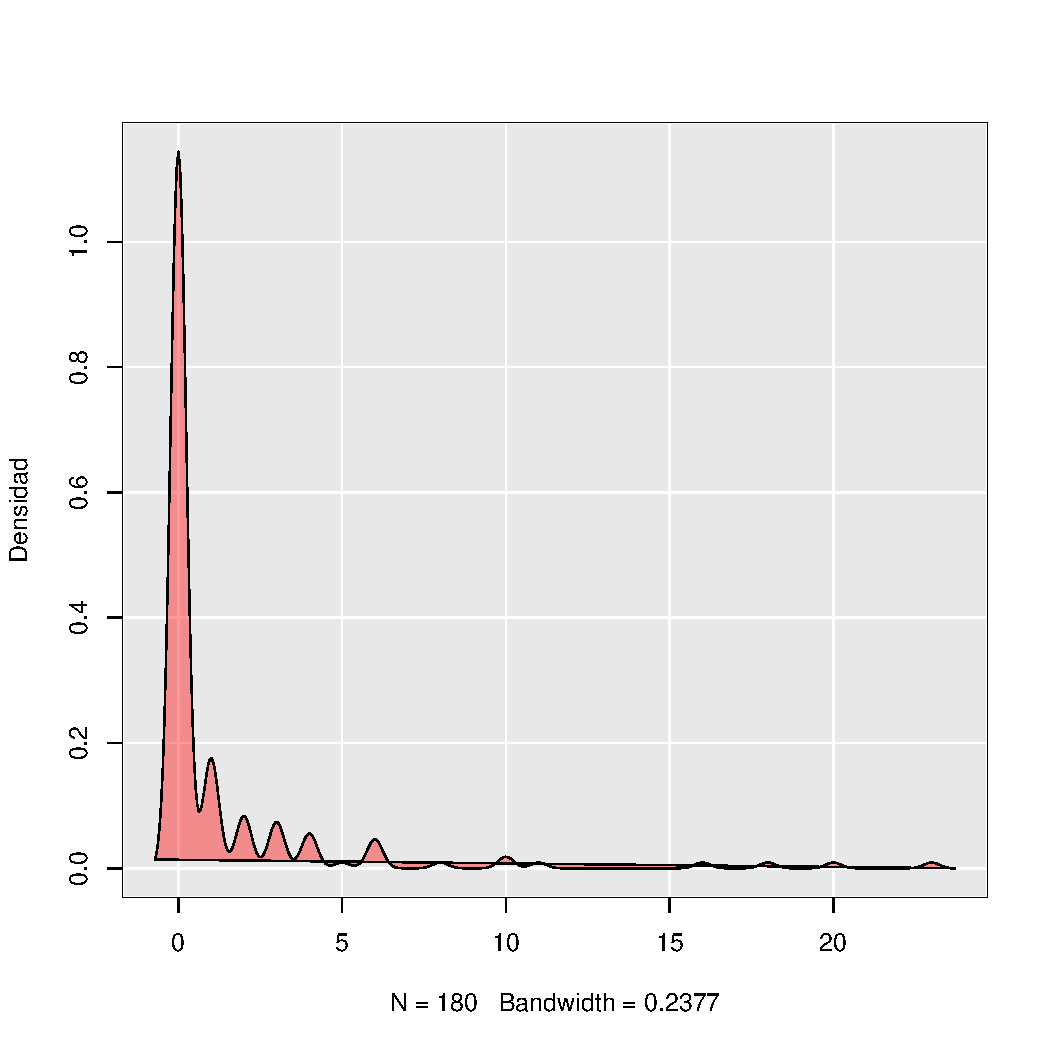
\includegraphics[width=\maxwidth]{figure/unnamed-chunk-41-1} \caption[Serie incendios]{Serie incendios: selección de modelos AIC y BIC.}\label{fig:unnamed-chunk-41}
\end{figure}


\end{knitrout}

A continuación se muestran las estimaciones de la matriz de transición de probabilidad $A$ para el ZIP HMM de orden 4, junto con el vector de medias de los estados dependientes $\lambda$, la distribución estacionaria $\pi$ y el parámetro de proporción de cero inflación $\theta$. De estos resultados observamos que al si se está en el estado 1 y lo más probables es seguir en este mismo estado con un valor de $82 \%$, mientras lo más improbables es pasar del estado 1 al 4 con apenas un $0.001 \%$. Para el ZIP HMM estacionario de orden 4, lo más factible es iniciar en el estado 2 con un $97 \%$, y como indica la tpm después pasar al estado 2 con un $48 \%$ de probabilidad. Asumiendo solo cero inflación en el estado 1, $\theta$ indica la proporción de cero GIF es de $44 \%$.



$$
A = \begin{pmatrix}{}
  0.820 & 0.154 & 0.025 & 0.001 \\ 
  0.483 & 0.335 & 0.131 & 0.050 \\ 
  0.168 & 0.329 & 0.499 & 0.004 \\ 
  0.004 & 0.329 & 0.346 & 0.320 \\ 
  \end{pmatrix}
$$

$$\lambda = (2.763, 15.114, 43.147, 99.306) \ \ \ \ \pi = (0.002, 0.997, 0.001, 0.000) \ \ \ \ \theta = 0.4440 $$



% latex table generated in R 3.6.0 by xtable 1.8-4 package
% Sun Jul 14 00:14:17 2019
\begin{table}[ht]
\centering
\scalebox{0.85}{
\begin{tabular}{rrrrrrrrrrrrrrrrrrrrrrrrrrrrrr}
  \hline
  \hline
2 & 2 & 2 & 1 & 1 & 1 & 1 & 1 & 1 & 1 & 1 & 1 & 1 & 1 & 2 & 1 & 1 & 1 & 1 & 1 & 1 & 1 & 1 & 1 & 1 & 2 & 2 & 1 & 1 & 1 \\ 
  1 & 2 & 1 & 1 & 1 & 1 & 1 & 1 & 2 & 1 & 1 & 1 & 1 & 2 & 2 & 1 & 1 & 1 & 1 & 1 & 1 & 1 & 1 & 1 & 1 & 1 & 2 & 1 & 1 & 1 \\ 
  2 & 4 & 2 & 1 & 1 & 1 & 1 & 1 & 1 & 1 & 1 & 1 & 1 & 1 & 1 & 1 & 1 & 1 & 1 & 1 & 1 & 1 & 1 & 1 & 1 & 1 & 1 & 1 & 1 & 1 \\ 
  2 & 2 & 3 & 2 & 1 & 2 & 4 & 4 & 3 & 1 & 1 & 1 & 1 & 1 & 1 & 1 & 1 & 1 & 2 & 2 & 1 & 1 & 1 & 1 & 1 & 2 & 2 & 1 & 1 & 1 \\ 
  2 & 2 & 2 & 1 & 1 & 1 & 3 & 3 & 3 & 1 & 1 & 1 & 3 & 3 & 3 & 2 & 1 & 1 & 2 & 2 & 3 & 2 & 1 & 1 & 2 & 3 & 2 & 2 & 1 & 1 \\ 
  3 & 3 & 3 & 1 & 1 & 1 & 2 & 2 & 2 & 1 & 2 & 1 & 2 & 3 & 3 & 2 & 1 & 2 & 3 & 3 & 3 & 2 & 1 & 1 & 1 & 2 & 2 & 1 & 1 & 1 \\ 
   \hline
\end{tabular}
}
\caption{Resultados de la decodificación global con el algoritmo Viterbi, para el ZIP HMM.} 
\end{table}


\begin{knitrout}
\definecolor{shadecolor}{rgb}{0.91, 0.91, 0.91}\color{fgcolor}\begin{figure}
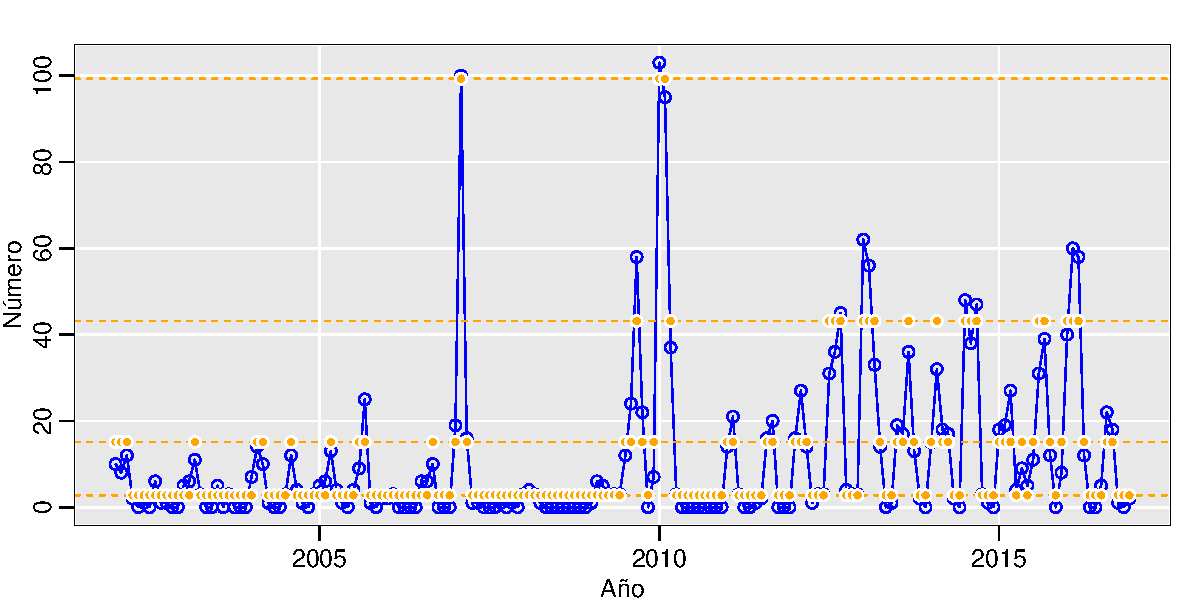
\includegraphics[width=\maxwidth]{figure/unnamed-chunk-45-1} \caption[Algoritmo Viterbi aplicado al ZIPHMM de tres estados]{Algoritmo Viterbi aplicado al ZIPHMM de tres estados.}\label{fig:unnamed-chunk-45}
\end{figure}


\end{knitrout}

La decodificación global se muestra en la tabla 16 y figura 15. Se observa que el estado 4 con una media de 99, sol hay 3 observaciones correspondientes a los GIF de febrero del 2007, enero del 2010 y febrero del 2010, mientras que el estado 3 con una media de 43 indica que estos 18 incendios la mayoría ocurrieron en tercer semestre, es decir en los meses julio, agosto y septiembre. Para el estado 2 con una media de 15 la mayoria de estos incendios ocurrieron en el primer semestre, finalmente para el estado 1 con una media de 2.8, se observa que en el último trimestre fue donde en su mayoría no ocurrieron GIF. Es así como el algoritmo Viterbi nos indica efectivamente que la serie tiene perídos estacionales.





\vspace{5mm} %5mm vertical space

\subsubsection*{Estimación Bayesiana del ZIP HMM}

Analogamente al caso de la serie homicidios a la cual se ajusto un PHMM, para la serie de homicidios se determinara el modelo más apropiado utilizanddo el factor de bayes. Para esto se ajustaron un total de seis modelos con estados 2, 3, 4, 5, 6 y 7. Como vimos anteriormente el factor de Bayes permite evaluar los datos a favor de una hipótesis nula y utilzar información externa para hacerlo. Dando peso de la evidencia a favor de una hipótesis dada.

Utilizando la notación del factor de Bayes que notamos como $B_{01}$ al contrastar dos hipótesis, $H_0$ (la hipótesis nula) y $H_1$ (la hipótesis alternativa), que se defini matemáticamente como:

$$B_{01} = \frac{\text{verosimilitud de los datos dado $H_0$}}{\text{verosimilitud de los datos dado $H_1$}} = \frac{P(D | H_0)}{P(D | H_1)}$$

Utilizando otra vez la interpretación propuesta por primera vez por Harold Jeffereys(1961) y modificada ligeramente por Lee y Wagenmakers en 2013, que está en la tabla 8, se deduce lo siguiente.

% latex table generated in R 3.6.0 by xtable 1.8-4 package
% Sun Jul 14 00:14:18 2019
\begin{table}[ht]
\centering
\begin{tabular}{rrrrrrr}
  \hline
 & mod 2 Est. & mod 3 Est. & mod 4 Est. & mod 5 Est. & mod 6 Est. & mod 7 Est. \\ 
  \hline
mod 2 Est. &  & 0.00 & 0.00 & 0.00 & 0.00 & 0.00 \\ 
  mod 3 Est. &  &  & 0.00 & 0.00 & 0.00 & 0.00 \\ 
  mod 4 Est. &  &  &  & 0.02 & 1.78 & 1513518.00 \\ 
  mod 5 Est. &  &  &  &  & 81.23 & 84986740.00 \\ 
  mod 6 Est. &  &  &  &  &  & 956226.00 \\ 
   \hline
\end{tabular}
\caption{Comparación resultados Factor de Bayes para los ZIP HMM.} 
\end{table}


Recordemos que las filas de la tabla x corresponden a $H_0$ y las columnas son $H_1$. Los resultados indican que tanto el modelo de 2 como el de 3 estados no son apropiados, pues el valor de 0 indica evidencia extrema para $H_1$. Por otra parte los resultados para el modelo de 4 estados, indican que es más apropiado que el de 6 y 7 estados, más no que el de 5 estados. Finalmente los modelos de 5 y 6 estados resultaron vencedores en sus contrastes. Lo que finalmente se concluye que el ZIP HMM más apropiado es el de 5 estados y en segundo lugar el ZIP HMM de orden 4.



Con el fin de comparar los resultados obtenidas de las estimaciones del ZIP HMM clásico vs el bayesiano, se decide ajustar el modelo con 4 estados. La salida que arroja Stan, en primer lugar la media de las estimaciones para los 21 parámetros más lp, el error y la desviación estándar que para este caso son bastante pequeños, seguidos de los intervalos de credibilidad alrededor de la media y a mediana que es casi identica a los valores de la media especialmnte para $\theta$ el parámetro de cero inflación y para el vector de medias, en la tpm varia ligeramente en algunos de los parámetros. Para este modelo se ajustaron 2.000 iteraciones con tres cadenas, la mitad de ellas se queman como calentamiento es decir que el número máximo de muestras efectivas debiera ser de 3.000, sin embargo ocurre algo extraño en varios de los parámetros $n\_eff > N$. Según el manual de Stan esto significa que los muestras que prroduce Stan son mejores que las muestras independientes para esos parámetros, o en otras palabras eel muestreo realizado por NUTS es súper eficiente, antitético y con sobre relajación (Geyer, 2011), esto ocurre porque en cada iteración es eliminada la correlación entre las muestras lo cual ocurre en casos extremadamente raros, para más información revise el manual o foro de Stan. Finalmente Gelman indica que el tamaño de muestra efectivo utilizados es el adecuado si Rhat es menor a 1.1, es decir que en este caso el muestreo fue óptimo.

% latex table generated in R 3.6.0 by xtable 1.8-4 package
% Sun Jul 14 00:14:18 2019
\begin{table}[ht]
\centering
\scalebox{0.95}{
\begin{tabular}{rrrrrrrrrrr}
  \hline
 & Media & Err.Sta & Desv & 2.5\% & 25\% & 50\% & 75\% & 97.5\% & n\_eff & Rhat \\ 
  \hline
$\theta$ & 0.449 & 0.001 & 0.050 & 0.351 & 0.414 & 0.449 & 0.483 & 0.545 & 5219.355 & 0.999 \\ 
  $\lambda_1$ & 2.868 & 0.004 & 0.266 & 2.371 & 2.684 & 2.866 & 3.047 & 3.408 & 4810.999 & 0.999 \\ 
  $\lambda_2$ & 15.369 & 0.012 & 0.775 & 13.859 & 14.830 & 15.361 & 15.874 & 16.877 & 4492.668 & 0.999 \\ 
  $\lambda_3$ & 43.153 & 0.040 & 1.807 & 39.600 & 42.040 & 43.143 & 44.300 & 46.658 & 2036.872 & 1.001 \\ 
  $\lambda_4$ & 99.235 & 0.145 & 6.120 & 87.428 & 95.445 & 99.219 & 103.236 & 110.912 & 1790.696 & 1.001 \\ 
  $a_{11}$ & 0.795 & 0.001 & 0.037 & 0.719 & 0.772 & 0.797 & 0.821 & 0.861 & 4587.670 & 0.999 \\ 
  $a_{12}$ & 0.158 & 0.000 & 0.034 & 0.098 & 0.134 & 0.156 & 0.180 & 0.231 & 4676.747 & 0.999 \\ 
  $a_{13}$ & 0.034 & 0.000 & 0.017 & 0.009 & 0.022 & 0.032 & 0.044 & 0.076 & 4870.506 & 1.000 \\ 
  $a_{14}$ & 0.013 & 0.000 & 0.011 & 0.000 & 0.005 & 0.010 & 0.018 & 0.040 & 3815.711 & 0.999 \\ 
  $a_{21}$ & 0.470 & 0.001 & 0.079 & 0.318 & 0.415 & 0.469 & 0.523 & 0.630 & 5238.938 & 0.999 \\ 
  $a_{22}$ & 0.328 & 0.001 & 0.077 & 0.192 & 0.272 & 0.325 & 0.380 & 0.482 & 5096.108 & 0.999 \\ 
  $a_{23}$ & 0.146 & 0.001 & 0.058 & 0.053 & 0.104 & 0.140 & 0.183 & 0.274 & 4306.099 & 1.000 \\ 
  $a_{24}$ & 0.056 & 0.001 & 0.037 & 0.008 & 0.029 & 0.049 & 0.076 & 0.147 & 4611.951 & 1.000 \\ 
  $a_{31}$ & 0.188 & 0.001 & 0.082 & 0.056 & 0.127 & 0.179 & 0.238 & 0.376 & 5736.173 & 1.000 \\ 
  $a_{32}$ & 0.331 & 0.001 & 0.099 & 0.151 & 0.261 & 0.325 & 0.396 & 0.537 & 5985.893 & 0.999 \\ 
  $a_{33}$ & 0.436 & 0.001 & 0.100 & 0.249 & 0.367 & 0.434 & 0.504 & 0.634 & 5179.787 & 1.000 \\ 
  $a_{34}$ & 0.045 & 0.001 & 0.043 & 0.001 & 0.013 & 0.032 & 0.063 & 0.161 & 3481.429 & 1.000 \\ 
  $a_{41}$ & 0.137 & 0.002 & 0.119 & 0.004 & 0.045 & 0.102 & 0.200 & 0.435 & 4984.285 & 0.999 \\ 
  $a_{42}$ & 0.309 & 0.002 & 0.163 & 0.055 & 0.182 & 0.287 & 0.421 & 0.658 & 5002.104 & 0.999 \\ 
  $a_{43}$ & 0.280 & 0.002 & 0.162 & 0.041 & 0.155 & 0.253 & 0.388 & 0.639 & 4855.509 & 1.000 \\ 
  $a_{44}$ & 0.274 & 0.002 & 0.157 & 0.037 & 0.152 & 0.252 & 0.376 & 0.630 & 4757.794 & 0.999 \\ 
  lp & -565.076 & 0.096 & 3.098 & -572.077 & -566.969 & -564.699 & -562.881 & -559.905 & 1032.526 & 1.007 \\ 
   \hline
\end{tabular}
}
\caption{Estimación bayesiana de los parámetros para un ZIPH-MM.} 
\end{table}


El gráfico de traza proporcionan una forma visual para inspeccionar el comportamiento de muestreo en cada uno de los parámetros de forma independiente y evaluar la mezcla a través de las cadenas y la convergencia, los resultados obtenidos para los 21 parámetros indican que se comportan de forma estable, ya que los valores muestreados en su mayoria se encuentran n un rango dee valores alrededor de la media. Dado el caso de la no convergencia el algunos casos la solución será aumentar el número de muestras.

\begin{knitrout}
\definecolor{shadecolor}{rgb}{0.91, 0.91, 0.91}\color{fgcolor}\begin{figure}
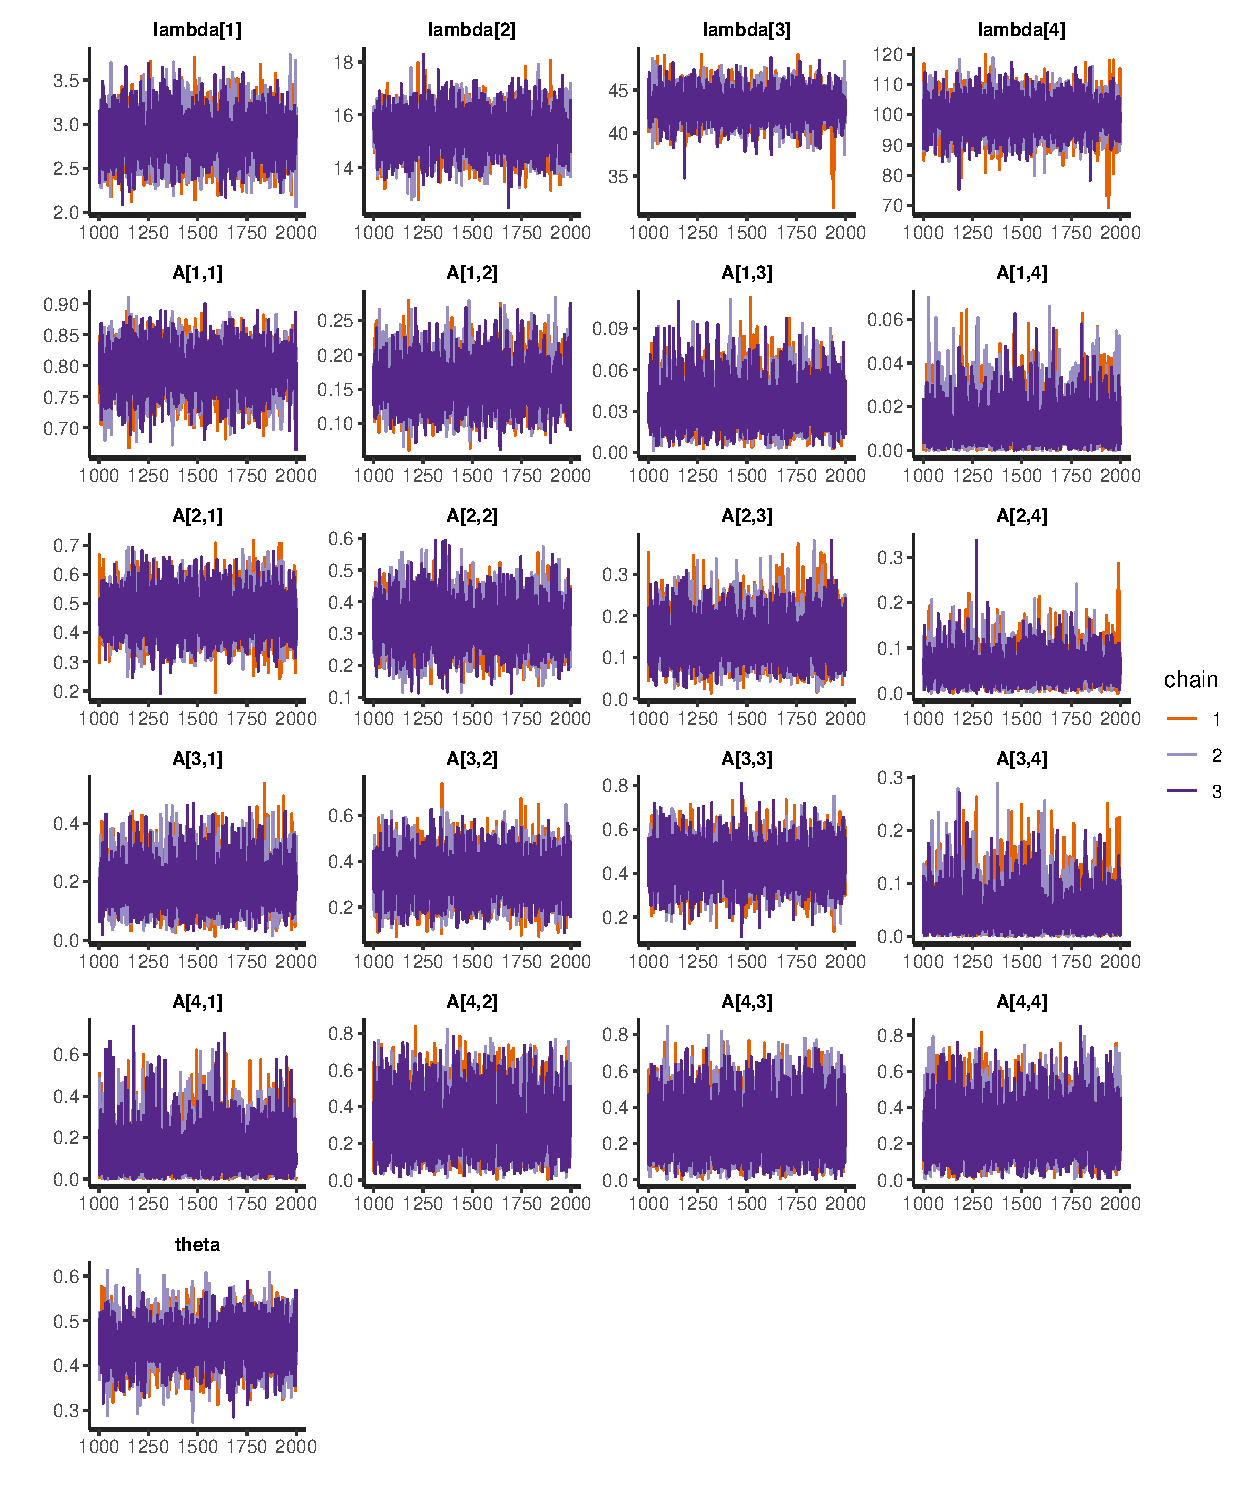
\includegraphics[width=\maxwidth]{figure/unnamed-chunk-51-1} \caption[Gráfico de trazas de las cadenas, para cada iteración y por cadena]{Gráfico de trazas de las cadenas, para cada iteración y por cadena.}\label{fig:unnamed-chunk-51}
\end{figure}


\end{knitrout}

En la estadísticas bayesianas, un intervalo creíble es un intervalo dentro del cual un valor de parámetro no observado cae con una probabilidad subjetiva particular. Es un intervalo en el dominio de una distribución de probabilidad posterior o una distribución predictiva. El intervalo e credibilidad es el equivalentebayesiano del intervalo de confianza no obstante, este depende de una distribución prior. Otra diferencia importante es que mientras en el intervalo de confianza se trata el parámetro como un valor fijo y los límites son variables aleatorias; en los intervalos creíbles, el parámetro estimado se trata como una variable aleatoria mientras que los límites se consideran fijos.
\\
Los intervalos de credibilidad al $95 \%$ calculados para la estimación de los parámetros del ZIP HMM, se encuentran en la figura 18. En la gráfica de la izquierda se encuentra el parámetro de cero inflación $\theta$, junto con las entradas de la matriz de transición $\gamma_{ij}$, ya que todos estos se encuentran en la misma escala, es decir se mueven entre cero y uno, mientras que el vector de medias $\lambda > 0$, se dibujo en el grafico de la derecha. Se encontraron intervalos bastante compactos, es decir que la longitud del intervalo es pequeña en la mayoría de los casos, exceptuando las fila tres y cuatro de la tpm, que presentan una asimetría y una dispersión considerable. Los intervalos nos permiten un uso práctico de que tan precisas son las estimaciones.
\\
El paquete bayesplot, proporciona la funciona MCMC-intervals basada en el método cuantil, que estima a partir de las muestras posterior los intervalos de credibilidad con un nivel de probabilidad fijado por el usuario. Por lo tanto su implementación es bastante sencilla.

\begin{knitrout}
\definecolor{shadecolor}{rgb}{0.91, 0.91, 0.91}\color{fgcolor}\begin{figure}
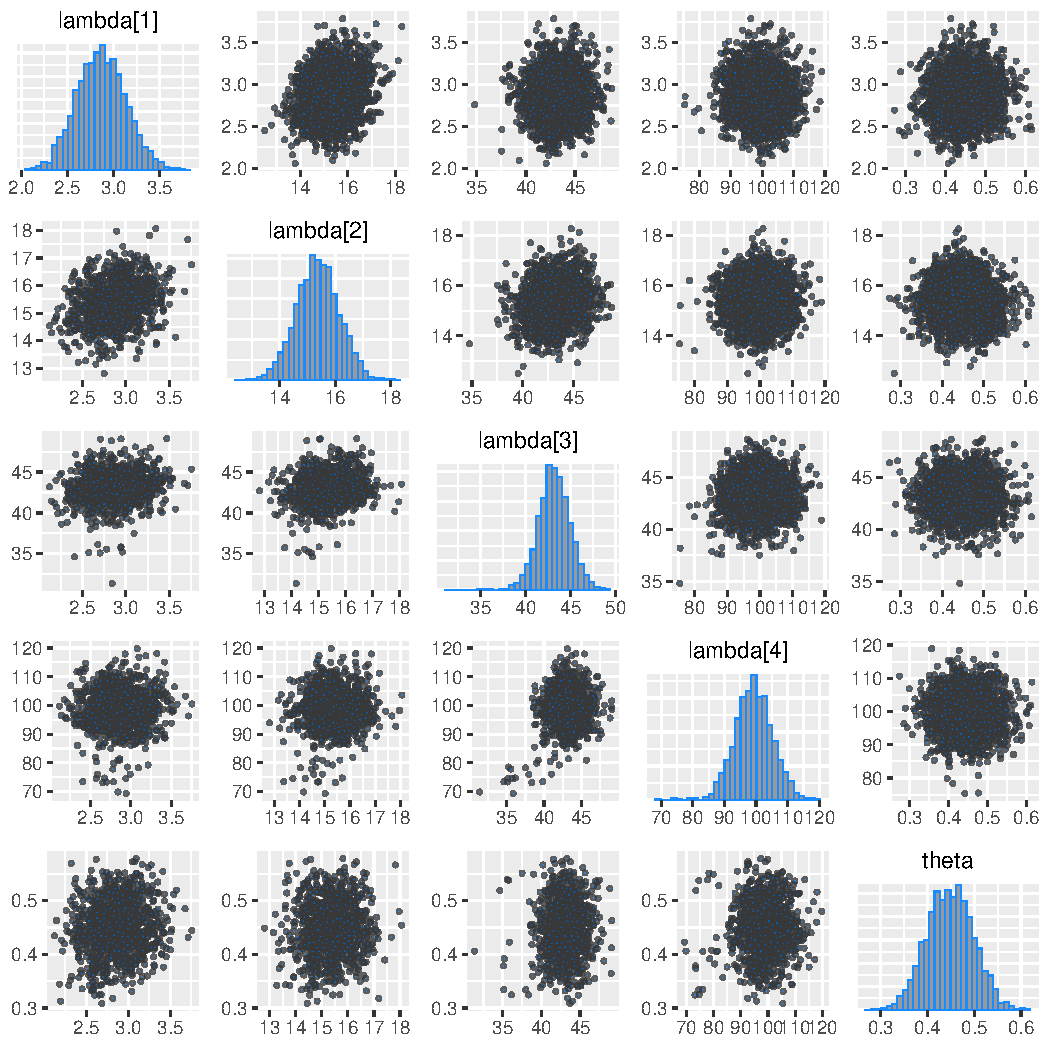
\includegraphics[width=\maxwidth]{figure/unnamed-chunk-52-1} \caption[Gráfico de dispersión para las muestras MCMC del ZIP HMM]{Gráfico de dispersión para las muestras MCMC del ZIP HMM.}\label{fig:unnamed-chunk-52}
\end{figure}


\end{knitrout}

En la figura 17 se graficaron los histogramas univariados y los diagramas de dispersión bivariados para el vector de medias de los estados dependientes y el parámetro de cero inflación, el gráfico para los parámetros restantes se adjunta en anexos. No se evidencian problemas de colinealidad, ni la presencia de no-identificabilidad multiplicativa (formas tipo plátano), o en términos más simples problemas de divergencias al momento de aplicar el No-U-Turn-Sampler (NUTS), asegurandonos que las inferencias sean apropiadas. Mientras que para la matriz de transición de probabilidad, parece haber problemas de colinealidad entre $\gamma_{11}$ con $\gamma_{12}$, y una ligera colinealidad entre $\gamma_{21}$ con $\gamma_{22}$ más no parecen haber problemas de no identificabilidad. Además se debe tener en cuenta que dada la restricción $\sum_{j=1}^m \gamma_{ij} = 1$, esto hace que los parámetros por fila de la tpm sean dependientes entre si, sin embargo a continuación se realizan pruebas más avanzadas como el Test de Heidel con el fin de determinar que los valores muestreados sean apropiados.

\begin{knitrout}
\definecolor{shadecolor}{rgb}{0.91, 0.91, 0.91}\color{fgcolor}\begin{figure}
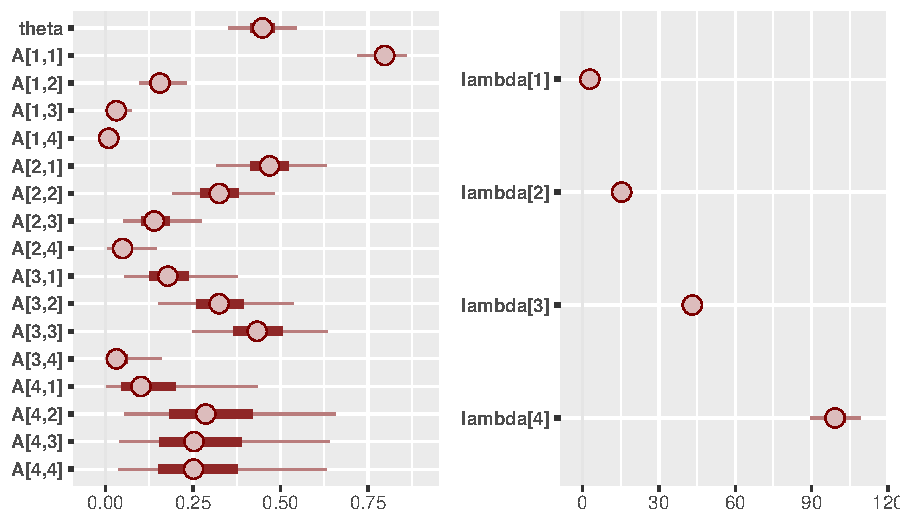
\includegraphics[width=\maxwidth]{figure/unnamed-chunk-53-1} \caption[Intervalos de crédibilidad al 0.95 ZIP HMM]{Intervalos de crédibilidad al 0.95 ZIP HMM.}\label{fig:unnamed-chunk-53}
\end{figure}


\end{knitrout}

% latex table generated in R 3.6.0 by xtable 1.8-4 package
% Sun Jul 14 00:14:29 2019
\begin{table}[ht]
\centering
\begin{tabular}{rlrlrr}
  \hline
 & P. Estacionariedad & Valor p & Prueba & Media & Medio.Ancho \\ 
  \hline
$\theta$ & páso & 0.928 & páso & 0.449 & 0.001 \\ 
  $\lambda_1$ & páso & 0.645 & páso & 2.868 & 0.008 \\ 
  $\lambda_2$ & páso & 0.689 & páso & 15.369 & 0.023 \\ 
  $\lambda_3$ & páso & 0.477 & páso & 43.153 & 0.080 \\ 
  $\lambda_4$ & páso & 0.594 & páso & 99.464 & 0.194 \\ 
  $a_{11}$ & páso & 0.601 & páso & 0.795 & 0.001 \\ 
  $a_{21}$ & páso & 0.504 & páso & 0.470 & 0.002 \\ 
  $a_{31}$ & páso & 0.257 & páso & 0.188 & 0.002 \\ 
  $a_{41}$ & páso & 0.611 & páso & 0.137 & 0.003 \\ 
  $a_{12}$ & páso & 0.444 & páso & 0.158 & 0.001 \\ 
  $a_{22}$ & páso & 0.356 & páso & 0.328 & 0.002 \\ 
  $a_{32}$ & páso & 0.620 & páso & 0.331 & 0.002 \\ 
  $a_{42}$ & páso & 0.992 & páso & 0.309 & 0.004 \\ 
  $a_{13}$ & páso & 0.632 & páso & 0.034 & 0.000 \\ 
  $a_{23}$ & páso & 0.786 & páso & 0.146 & 0.002 \\ 
  $a_{33}$ & páso & 0.091 & páso & 0.436 & 0.003 \\ 
  $a_{43}$ & páso & 0.462 & páso & 0.280 & 0.004 \\ 
  $a_{14}$ & páso & 0.765 & páso & 0.012 & 0.000 \\ 
  $a_{24}$ & páso & 0.234 & páso & 0.056 & 0.001 \\ 
  $a_{34}$ & páso & 0.268 & páso & 0.045 & 0.001 \\ 
  $a_{44}$ & páso & 0.583 & páso & 0.274 & 0.004 \\ 
  lp & páso & 0.175 & páso & -564.870 & 0.207 \\ 
   \hline
\end{tabular}
\caption{Prueba de estacionariedad, usando el estadístico de Cramer-von-Mises para la convergencia de la cadena y prueba de medio ancho para la media calculando el intervalo de confianza al 0.95.} 
\end{table}


Con el fin de establecer técnicas más sofisticadas para determinar si el proceso de muestreo por NUTS, fue exitosos existen diferentes metodologías, tanto gráficas como basadas en hipótesis. La gráfica de traza en la figura 16 parece consistente, sin embargo la prueba de convergencia de Heidel, permite determinar si los valores muestreados provienen de una distribución estacionaria. Por lo tanto se aplica esta prueba para cada uno de los parámetros obtenidos por el ZIP HMM y se contrasta contrastan con la estadística de Cramer-von-Mises para un nivel de significancia $\alpha = 0.05$ fijo, donde la hipótesis nula es que la cadena es estacionaria. En todos los casos el valor p fue mayor que 0.05 lo que indica que existe suficiente evidencia estadística para no rechazar la hipótesis nula, lo cual indica que los valores muestreados ofrecen una estimación confiable al provenir de una distribución estacionaria. 
También se utilizo la prueba de medio ancho, que calcula un intervalo de confianza del $95 \%$ para la media, y utiliza la parte de la cadena que pasó la prueba de estacionariedad, para determinar si la muestra fue lo suficientemente grande para estimar la media con precisión. Los resultados indican que efectivamente cada uno de los parámetros aprobo la prueba de medio ancho.

\clearpage

\subsubsection{Comparación ZIP HMM clásico vs Bayesiano}

Igual que en el caso del PHMM, la estimación bajo el enfoque clásico se realizo utilizando bootstrap, generando 100 muestras independientes a partir del ZIP HMM de orden 4 de longitud 180 igual a la serie GIF en Colombia. Los valores iniciales usados fueron los estimados por ZIP HMM de 4 estados, que permiten la convergencia del algoritmo en pocas iteraciones. La probabilidad y el nivel deconfianza se fijo al 0.95, para los intervalos de credibilidad y confianza, respectivamente, en la tabla 20 se encuentran rgistrados los resultados obtenidos.
\\
Ambos intervalos se relacionan con la precisión de nuestra estimación. La forma más comun para saber el desempeño del método, es calculando la longitud de este, donde se espera que el ancho sea lo más pequeño posible. Los resultados se muestran en la tabla 20, junto con la media de las estimaciones, tanto para el ZIP HMM frecuentista como para el bayesoano. No parece haber un ganador indiscutible, si embargo haciendo un análisis más detallado por parámetros se puede decir lo siguiente. Para $\theta$ el parámetro de cero inflación es más pequeña la longitud en el caso bayesiano, para el vetor de medias $\lambda$ es un empate 2 y 2 para cada uno, sin embargo preocupa que para $\lambda_4$ en el caso clásico el ancho es extremadamente grande. Finalmente para los valores de la tpm en 9 de los 16 intervalos estimados, el enfoque bayesiano nuevamente es el vencedor. En conclusión aunque el los intervalos de credibilidad tienen una longitud en la mayoría de los casos, no parece haber un método que sea evidentemente el mejor.





% latex table generated in R 3.6.0 by xtable 1.8-4 package
% Sun Jul 14 00:14:29 2019
\begin{table}[ht]
\centering
\begin{tabular}{lrrrrrrrr}
  \toprule
   & \multicolumn{4}{c}{\textbf{Intervalos de Credibilidad}} & \multicolumn{4}{c}{\textbf{Intervalos de Confianza}}\\
 \cmidrule(lr){2-5}\cmidrule(lr){6-9}
 \textbf{Parámetros} & \textbf{Media} & \textbf{2.5} & \textbf{97.5} & \textbf{Ancho} & \textbf{Media} & \textbf{2.5} & \textbf{97.5} & \textbf{Ancho}\\
 \midrule
$\theta$ & 0.449 & 0.351 & 0.545 & 0.194 & 0.444 & 0.343 & 0.543 & 0.200 \\ 
  $\lambda_1$ & 2.868 & 2.371 & 3.408 & 1.037 & 2.763 & 2.218 & 3.181 & 0.963 \\ 
  $\lambda_2$ & 15.369 & 13.859 & 16.877 & 3.017 & 15.115 & 13.853 & 16.409 & 2.556 \\ 
  $\lambda_3$ & 43.153 & 39.600 & 46.658 & 7.059 & 43.148 & 40.002 & 46.844 & 6.842 \\ 
  $\lambda_4$ & 99.235 & 87.428 & 110.912 & 23.485 & 99.306 & 38.082 & 109.076 & 70.994 \\ 
  $a_{11}$ & 0.795 & 0.719 & 0.861 & 0.142 & 0.820 & 0.735 & 0.889 & 0.154 \\ 
  $a_{21}$ & 0.470 & 0.318 & 0.630 & 0.313 & 0.483 & 0.317 & 0.680 & 0.363 \\ 
  $a_{31}$ & 0.188 & 0.056 & 0.376 & 0.320 & 0.168 & 0.019 & 0.366 & 0.347 \\ 
  $a_{41}$ & 0.137 & 0.004 & 0.435 & 0.431 & 0.004 & 0.000 & 0.006 & 0.006 \\ 
  $a_{12}$ & 0.158 & 0.098 & 0.231 & 0.133 & 0.154 & 0.089 & 0.221 & 0.131 \\ 
  $a_{22}$ & 0.328 & 0.192 & 0.482 & 0.290 & 0.335 & 0.184 & 0.500 & 0.316 \\ 
  $a_{32}$ & 0.331 & 0.151 & 0.537 & 0.386 & 0.329 & 0.128 & 0.643 & 0.514 \\ 
  $a_{42}$ & 0.309 & 0.055 & 0.658 & 0.603 & 0.329 & 0.000 & 0.996 & 0.996 \\ 
  $a_{13}$ & 0.034 & 0.009 & 0.076 & 0.067 & 0.025 & 0.001 & 0.065 & 0.064 \\ 
  $a_{23}$ & 0.146 & 0.053 & 0.274 & 0.221 & 0.131 & 0.051 & 0.257 & 0.206 \\ 
  $a_{33}$ & 0.436 & 0.249 & 0.634 & 0.385 & 0.499 & 0.210 & 0.665 & 0.455 \\ 
  $a_{43}$ & 0.280 & 0.041 & 0.639 & 0.598 & 0.346 & 0.000 & 0.998 & 0.997 \\ 
  $a_{14}$ & 0.013 & 0.000 & 0.040 & 0.039 & 0.001 & 0.000 & 0.018 & 0.018 \\ 
  $a_{24}$ & 0.056 & 0.008 & 0.147 & 0.140 & 0.050 & 0.004 & 0.138 & 0.134 \\ 
  $a_{34}$ & 0.045 & 0.001 & 0.161 & 0.160 & 0.004 & 0.000 & 0.099 & 0.099 \\ 
  $a_{44}$ & 0.274 & 0.037 & 0.630 & 0.593 & 0.320 & 0.000 & 0.665 & 0.665 \\ 
   \bottomrule
\end{tabular}
\caption{Intervalos de Credibilidad y Confianza para el ZIP HMM de orden 4.} 
\end{table}


\clearpage

\section{Anexo Códigos}

A continuación se anexa el código utilizado para el desarrollo de esta tesis, en la aplicación del PHMM a la base homicidios en Colombia y el ajuste del ZIP-HMM a los Grandes Incendios Forestales (GIF) en Colombia. 

\begin{knitrout}
\definecolor{shadecolor}{rgb}{0.91, 0.91, 0.91}\color{fgcolor}\begin{kframe}
\begin{alltt}
\hlkwd{rm}\hlstd{(}\hlkwc{list} \hlstd{=} \hlkwd{ls}\hlstd{())}
\hlcom{############ Packages #}
\hlkwd{library}\hlstd{(Bayeshmmcts)}
\hlkwd{library}\hlstd{(bridgesampling)}
\hlkwd{library}\hlstd{(rstan)}
\hlkwd{library}\hlstd{(bayesplot)}
\hlkwd{library}\hlstd{(coda)}
\hlkwd{library}\hlstd{(ziphsmm)}

\hlcom{##### Data homicidios #}
\hlkwd{data}\hlstd{(}\hlstr{"homicides"}\hlstd{)}

\hlcom{##### Poisson - Hidden Markov Model #}
\hlstd{homicidios} \hlkwb{<-} \hlstd{homicides}
\hlkwd{colnames}\hlstd{(homicidios)} \hlkwb{<-} \hlkwd{c}\hlstd{(}\hlstr{"Año"}\hlstd{,} \hlstr{"Homicidios"}\hlstd{,} \hlstr{"Población"}\hlstd{,} \hlstr{"Tasa"}\hlstd{)}
\hlstd{Homicidios} \hlkwb{<-} \hlkwd{ts}\hlstd{(}\hlkwc{data} \hlstd{=} \hlkwd{round}\hlstd{(homicidios}\hlopt{$}\hlstd{Tasa),} \hlkwc{start} \hlstd{=} \hlnum{1960}\hlstd{)}

\hlcom{# modelo clasico}
\hlstd{mod2} \hlkwb{<-} \hlkwd{pois.HMM.mle}\hlstd{(}\hlkwc{o} \hlstd{= Homicidios,} \hlkwc{m} \hlstd{=} \hlnum{2}\hlstd{,} \hlkwc{lambda0} \hlstd{=} \hlkwd{c}\hlstd{(}\hlnum{30}\hlstd{,} \hlnum{63}\hlstd{),} \hlkwc{A0} \hlstd{=} \hlkwd{matrix}\hlstd{(}\hlkwd{c}\hlstd{(}\hlnum{0.9}\hlstd{,}
    \hlnum{0.1}\hlstd{,} \hlnum{0.1}\hlstd{,} \hlnum{0.9}\hlstd{),} \hlnum{2}\hlstd{,} \hlnum{2}\hlstd{,} \hlkwc{byrow} \hlstd{=} \hlnum{TRUE}\hlstd{),} \hlkwc{stationary} \hlstd{=} \hlnum{TRUE}\hlstd{)}

\hlcom{# Algoritmo viterbi (decodificación Global)}
\hlstd{viterbi} \hlkwb{<-} \hlkwd{pois.HMM.viterbi}\hlstd{(}\hlkwc{o} \hlstd{= Homicidios,} \hlkwc{mod} \hlstd{= mod2)}

\hlcom{# Verificación de supuestos}
\hlstd{residuales} \hlkwb{<-} \hlkwd{pois.HMM.pseudo_residuals}\hlstd{(}\hlkwc{o} \hlstd{= Homicidios,} \hlkwc{mod} \hlstd{= mod2)}
\hlkwd{pois.HMM.plot.residuals}\hlstd{(residuales)}

\hlcom{# Predicción de los estados}
\hlstd{año} \hlkwb{<-} \hlstd{homicidios}\hlopt{$}\hlstd{Año}
\hlstd{Estad_pred} \hlkwb{<-} \hlkwd{data.frame}\hlstd{(}\hlkwc{Año} \hlstd{= año[}\hlnum{59}\hlstd{]} \hlopt{+} \hlnum{1}\hlopt{:}\hlnum{16}\hlstd{,} \hlkwd{pois.HMM.state_prediction}\hlstd{(}\hlkwc{h} \hlstd{=} \hlnum{16}\hlstd{,}
    \hlkwc{o} \hlstd{= Homicidios,} \hlkwc{mod} \hlstd{= mod2))}
\hlkwd{colnames}\hlstd{(Estad_pred)} \hlkwb{<-} \hlkwd{c}\hlstd{(}\hlstr{"Año"}\hlstd{,} \hlstr{"Estado 1"}\hlstd{,} \hlstr{"Estado 2"}\hlstd{)}
\hlstd{Estad_pred}\hlopt{$}\hlstd{Estado} \hlkwb{<-} \hlkwd{apply}\hlstd{(Estad_pred,} \hlnum{1}\hlstd{, which.max)}

\hlcom{# Distribución de prónostico}
\hlstd{delta} \hlkwb{<-} \hlkwd{pois.HMM.stadist}\hlstd{(mod2)}
\hlstd{h} \hlkwb{<-} \hlnum{16}
\hlstd{xf} \hlkwb{<-} \hlnum{5}\hlopt{:}\hlnum{75}
\hlstd{año} \hlkwb{<-} \hlstd{homicidios[,} \hlnum{1}\hlstd{]}
\hlstd{forecasts} \hlkwb{<-} \hlkwd{pois.HMM.forecast}\hlstd{(xf, h, Homicidios, mod2)}
\hlkwd{par}\hlstd{(}\hlkwc{mfrow} \hlstd{=} \hlkwd{c}\hlstd{(}\hlnum{4}\hlstd{,} \hlnum{4}\hlstd{),} \hlkwc{las} \hlstd{=} \hlnum{1}\hlstd{)}
\hlkwa{for} \hlstd{(i} \hlkwa{in} \hlnum{1}\hlopt{:}\hlstd{h) \{}
    \hlstd{fc} \hlkwb{<-} \hlstd{forecasts[, i]}
    \hlkwd{plot}\hlstd{(xf, fc,} \hlkwc{type} \hlstd{=} \hlstr{"h"}\hlstd{,} \hlkwc{main} \hlstd{=} \hlkwd{paste}\hlstd{(}\hlstr{"Dist. pronós."}\hlstd{, año[}\hlnum{59}\hlstd{]} \hlopt{+} \hlstd{i),} \hlkwc{xlim} \hlstd{=} \hlkwd{c}\hlstd{(}\hlnum{5}\hlstd{,}
        \hlkwd{max}\hlstd{(xf} \hlopt{+} \hlnum{2}\hlstd{)),} \hlkwc{ylim} \hlstd{=} \hlkwd{c}\hlstd{(}\hlnum{0}\hlstd{,} \hlnum{0.1}\hlstd{),} \hlkwc{cex.main} \hlstd{=} \hlnum{0.85}\hlstd{,} \hlkwc{xlab} \hlstd{=} \hlstr{"conteo"}\hlstd{,} \hlkwc{ylab} \hlstd{=} \hlstr{"probabilidad"}\hlstd{,}
        \hlkwc{lwd} \hlstd{=} \hlnum{1}\hlstd{)}
    \hlkwd{rect}\hlstd{(}\hlkwd{par}\hlstd{(}\hlstr{"usr"}\hlstd{)[}\hlnum{1}\hlstd{],} \hlkwd{par}\hlstd{(}\hlstr{"usr"}\hlstd{)[}\hlnum{3}\hlstd{],} \hlkwd{par}\hlstd{(}\hlstr{"usr"}\hlstd{)[}\hlnum{2}\hlstd{],} \hlkwd{par}\hlstd{(}\hlstr{"usr"}\hlstd{)[}\hlnum{4}\hlstd{],} \hlkwc{col} \hlstd{=} \hlkwd{gray}\hlstd{(}\hlnum{0.9}\hlstd{,}
        \hlnum{0.9}\hlstd{),} \hlkwc{border} \hlstd{=} \hlstr{"white"}\hlstd{)}
    \hlkwd{grid}\hlstd{(}\hlkwc{lty} \hlstd{=} \hlnum{1}\hlstd{,} \hlkwc{col} \hlstd{=} \hlstr{"white"}\hlstd{)}
    \hlkwd{lines}\hlstd{(xf, fc,} \hlkwc{type} \hlstd{=} \hlstr{"h"}\hlstd{,} \hlkwc{lwd} \hlstd{=} \hlnum{1}\hlstd{)}
    \hlstd{dstat} \hlkwb{<-} \hlkwd{numeric}\hlstd{(}\hlkwd{length}\hlstd{(xf))}
    \hlkwa{for} \hlstd{(j} \hlkwa{in} \hlnum{1}\hlopt{:}\hlstd{mod2}\hlopt{$}\hlstd{m) dstat} \hlkwb{<-} \hlstd{dstat} \hlopt{+} \hlstd{delta[j]} \hlopt{*} \hlkwd{dpois}\hlstd{(xf, mod2}\hlopt{$}\hlstd{lambda[j])}
    \hlkwd{lines}\hlstd{(xf, dstat,} \hlkwc{col} \hlstd{=} \hlstr{"chartreuse2"}\hlstd{,} \hlkwc{lwd} \hlstd{=} \hlnum{2}\hlstd{)}
\hlstd{\}}

\hlcom{# Modelo bayesiano de 2 estados}
\hlstd{PHMM_2states} \hlkwb{<-} \hlkwd{bayes.PHMM}\hlstd{(}\hlkwc{y} \hlstd{= Homicidios,} \hlkwc{m} \hlstd{=} \hlnum{2}\hlstd{,} \hlkwc{chains} \hlstd{=} \hlnum{3}\hlstd{,} \hlkwc{iter} \hlstd{=} \hlnum{2000}\hlstd{,} \hlkwc{control} \hlstd{=} \hlkwd{list}\hlstd{(}\hlkwc{adapt_delta} \hlstd{=} \hlnum{0.99}\hlstd{))}
\hlkwd{print}\hlstd{(PHMM_2states,} \hlkwc{digits} \hlstd{=} \hlnum{3}\hlstd{)}

\hlcom{# Modelo bayesiano de 3 estados}
\hlstd{PHMM_3states} \hlkwb{<-} \hlkwd{bayes.PHMM}\hlstd{(}\hlkwc{y} \hlstd{= Homicidios,} \hlkwc{m} \hlstd{=} \hlnum{3}\hlstd{,} \hlkwc{chains} \hlstd{=} \hlnum{3}\hlstd{,} \hlkwc{iter} \hlstd{=} \hlnum{2000}\hlstd{,} \hlkwc{control} \hlstd{=} \hlkwd{list}\hlstd{(}\hlkwc{adapt_delta} \hlstd{=} \hlnum{0.99}\hlstd{))}


\hlcom{# estimates of the log marginal likelihoods}
\hlstd{bridge_H0} \hlkwb{<-} \hlkwd{bridge_sampler}\hlstd{(}\hlkwc{samples} \hlstd{= PHMM_2states)}
\hlstd{bridge_H1} \hlkwb{<-} \hlkwd{bridge_sampler}\hlstd{(}\hlkwc{samples} \hlstd{= PHMM_3states)}

\hlkwd{error_measures}\hlstd{(bridge_H0)}\hlopt{$}\hlstd{percentage}
\hlkwd{error_measures}\hlstd{(bridge_H1)}\hlopt{$}\hlstd{percentage}

\hlcom{# The Bayes factor in favor of H0 over H1 can then be obtained as follows:}
\hlstd{bridge_H0}\hlopt{$}\hlstd{logml}
\hlstd{bridge_H1}\hlopt{$}\hlstd{logml}

\hlcom{# Factor de bayes}
\hlkwd{bf}\hlstd{(bridge_H0, bridge_H1)}

\hlcom{# Posterior}
\hlstd{posterior} \hlkwb{<-} \hlkwd{as.array}\hlstd{(PHMM_2states)}
\hlstd{lp_cp} \hlkwb{<-} \hlkwd{log_posterior}\hlstd{(PHMM_2states)}
\hlstd{np_cp} \hlkwb{<-} \hlkwd{nuts_params}\hlstd{(PHMM_2states)}
\hlstd{rstan}\hlopt{::}\hlkwd{traceplot}\hlstd{(PHMM_2states)}

\hlcom{# Gráfica de intevalos de credibilidad}
\hlkwd{color_scheme_set}\hlstd{(}\hlstr{"red"}\hlstd{)}
\hlkwd{mcmc_intervals}\hlstd{(posterior,} \hlkwc{prob_outer} \hlstd{=} \hlnum{0.95}\hlstd{,} \hlkwc{pars} \hlstd{=} \hlkwd{c}\hlstd{(}\hlstr{"A[1,1]"}\hlstd{,} \hlstr{"A[1,2]"}\hlstd{,} \hlstr{"A[2,1]"}\hlstd{,}
    \hlstr{"A[2,2]"}\hlstd{))}

\hlcom{# Histogragmas univariados y gráfico de dispersión bivariado}
\hlkwd{color_scheme_set}\hlstd{(}\hlstr{"mix-brightblue-gray"}\hlstd{)}
\hlkwd{mcmc_pairs}\hlstd{(posterior,} \hlkwc{np} \hlstd{= np_cp,} \hlkwc{pars} \hlstd{=} \hlkwd{c}\hlstd{(}\hlstr{"A[1,1]"}\hlstd{,} \hlstr{"A[1,2]"}\hlstd{,} \hlstr{"A[2,1]"}\hlstd{,} \hlstr{"A[2,2]"}\hlstd{,}
    \hlstr{"lambda[1]"}\hlstd{,} \hlstr{"lambda[2]"}\hlstd{),} \hlkwc{off_diag_args} \hlstd{=} \hlkwd{list}\hlstd{(}\hlkwc{size} \hlstd{=} \hlnum{0.75}\hlstd{))}

\hlcom{# Prueba de Heibelberg y test medio ancho}
\hlstd{PHMM_mcmc} \hlkwb{<-} \hlkwd{as.mcmc}\hlstd{(}\hlkwd{as.matrix}\hlstd{(PHMM_2states))}
\hlstd{Test_HyW} \hlkwb{<-} \hlkwd{heidel.diag}\hlstd{(PHMM_mcmc)}

\hlcom{# Intervalos de Confianza y de credibilidad}
\hlstd{intervalos_cred} \hlkwb{<-} \hlkwd{mcmc_intervals_data}\hlstd{(posterior,} \hlkwc{prob_outer} \hlstd{=} \hlnum{0.95}\hlstd{,} \hlkwc{point_est} \hlstd{=} \hlstr{"mean"}\hlstd{)}
\hlstd{intervalos_conf} \hlkwb{<-} \hlkwd{pois.HMM.confint}\hlstd{(}\hlkwc{mod} \hlstd{= mod2,} \hlkwc{n} \hlstd{=} \hlnum{59}\hlstd{,} \hlkwc{B} \hlstd{=} \hlnum{250}\hlstd{)}

\hlcom{##### Zero Inflated Poisson - Hidden Markov Model #}
\hlkwd{rm}\hlstd{(}\hlkwc{list} \hlstd{=} \hlkwd{ls}\hlstd{())}

\hlcom{##### Data GIF #}
\hlkwd{data}\hlstd{(}\hlstr{"wildfires"}\hlstd{)}
\hlstd{incendios} \hlkwb{<-} \hlstd{wildfires}
\hlkwd{colnames}\hlstd{(incendios)} \hlkwb{<-} \hlkwd{c}\hlstd{(}\hlstr{"Fecha"}\hlstd{,} \hlstr{"GIF"}\hlstd{)}
\hlstd{GIF} \hlkwb{<-} \hlkwd{ts}\hlstd{(}\hlkwc{data} \hlstd{= incendios}\hlopt{$}\hlstd{GIF,} \hlkwc{start} \hlstd{=} \hlkwd{c}\hlstd{(}\hlnum{2002}\hlstd{,} \hlnum{1}\hlstd{),} \hlkwc{frequency} \hlstd{=} \hlnum{12}\hlstd{)}

\hlcom{#### ZIP HMM clásico de 2 estados}
\hlstd{ZIPHMM_2states} \hlkwb{<-} \hlkwd{hmmfit}\hlstd{(}\hlkwc{y} \hlstd{= incendios}\hlopt{$}\hlstd{GIF,} \hlkwc{M} \hlstd{=} \hlnum{2}\hlstd{,} \hlkwc{prior_init} \hlstd{=} \hlkwd{c}\hlstd{(}\hlnum{0.6}\hlstd{,} \hlnum{0.4}\hlstd{),}
    \hlkwc{tpm_init} \hlstd{=} \hlkwd{matrix}\hlstd{(}\hlkwd{c}\hlstd{(}\hlnum{0.9}\hlstd{,} \hlnum{0.1}\hlstd{,} \hlnum{0.5}\hlstd{,} \hlnum{0.5}\hlstd{),} \hlnum{2}\hlstd{,} \hlnum{2}\hlstd{,} \hlkwc{byrow} \hlstd{=} \hlnum{TRUE}\hlstd{),} \hlkwc{emit_init} \hlstd{=} \hlkwd{c}\hlstd{(}\hlnum{7}\hlstd{,}
        \hlnum{45}\hlstd{),} \hlkwc{zero_init} \hlstd{=} \hlkwd{c}\hlstd{(}\hlnum{0.4}\hlstd{,} \hlnum{0}\hlstd{),} \hlkwc{method} \hlstd{=} \hlstr{"Nelder-Mead"}\hlstd{,} \hlkwc{hessian} \hlstd{=} \hlnum{TRUE}\hlstd{,}
    \hlkwc{control} \hlstd{=} \hlkwd{list}\hlstd{(}\hlkwc{maxit} \hlstd{=} \hlnum{1000}\hlstd{,} \hlkwc{trace} \hlstd{=} \hlnum{1}\hlstd{))}

\hlcom{#### ZIP HMM clásico de 4 estados}
\hlstd{ZIPHMM_4states} \hlkwb{<-} \hlkwd{hmmfit}\hlstd{(}\hlkwc{y} \hlstd{= incendios}\hlopt{$}\hlstd{GIF,} \hlkwc{M} \hlstd{=} \hlnum{4}\hlstd{,} \hlkwc{prior_init} \hlstd{=} \hlkwd{c}\hlstd{(}\hlnum{0.5}\hlstd{,} \hlnum{0.2}\hlstd{,}
    \hlnum{0.2}\hlstd{,} \hlnum{0.1}\hlstd{),} \hlkwc{tpm_init} \hlstd{=} \hlkwd{matrix}\hlstd{(}\hlkwd{c}\hlstd{(}\hlnum{0.8}\hlstd{,} \hlnum{0.15}\hlstd{,} \hlnum{0.04}\hlstd{,} \hlnum{0.01}\hlstd{,} \hlnum{0.5}\hlstd{,} \hlnum{0.3}\hlstd{,} \hlnum{0.15}\hlstd{,} \hlnum{0.05}\hlstd{,}
    \hlnum{0.15}\hlstd{,} \hlnum{0.35}\hlstd{,} \hlnum{0.45}\hlstd{,} \hlnum{0.05}\hlstd{,} \hlnum{0.15}\hlstd{,} \hlnum{0.35}\hlstd{,} \hlnum{0.25}\hlstd{,} \hlnum{0.25}\hlstd{),} \hlnum{4}\hlstd{,} \hlnum{4}\hlstd{,} \hlkwc{byrow} \hlstd{=} \hlnum{TRUE}\hlstd{),} \hlkwc{emit_init} \hlstd{=} \hlkwd{c}\hlstd{(}\hlnum{3}\hlstd{,}
    \hlnum{15}\hlstd{,} \hlnum{43}\hlstd{,} \hlnum{100}\hlstd{),} \hlkwc{zero_init} \hlstd{=} \hlkwd{c}\hlstd{(}\hlnum{0.45}\hlstd{,} \hlnum{0}\hlstd{,} \hlnum{0}\hlstd{,} \hlnum{0}\hlstd{),} \hlkwc{method} \hlstd{=} \hlstr{"Nelder-Mead"}\hlstd{,} \hlkwc{hessian} \hlstd{=} \hlnum{TRUE}\hlstd{,}
    \hlkwc{control} \hlstd{=} \hlkwd{list}\hlstd{(}\hlkwc{maxit} \hlstd{=} \hlnum{1000}\hlstd{,} \hlkwc{trace} \hlstd{=} \hlnum{1}\hlstd{))}

\hlcom{# Algoritmo Viterbi para el ZIP HMM}
\hlstd{ZIP.viterbi} \hlkwb{<-} \hlkwd{hmmviterbi}\hlstd{(}\hlkwc{y} \hlstd{= incendios}\hlopt{$}\hlstd{GIF,} \hlkwc{ntimes} \hlstd{=} \hlkwd{length}\hlstd{(incendios}\hlopt{$}\hlstd{GIF),}
    \hlkwc{M} \hlstd{=} \hlnum{4}\hlstd{,} \hlkwc{prior_init} \hlstd{= ZIPHMM_4states}\hlopt{$}\hlstd{prior,} \hlkwc{tpm_init} \hlstd{= ZIPHMM_4states}\hlopt{$}\hlstd{tpm,}
    \hlkwc{emit_init} \hlstd{= ZIPHMM_4states}\hlopt{$}\hlstd{emit_parm,} \hlkwc{zero_init} \hlstd{= ZIPHMM_4states}\hlopt{$}\hlstd{zeroprop)}

\hlcom{# Grráfica ddeecodificación algoritmo Viterbi}
\hlkwd{par}\hlstd{(}\hlkwc{mfrow} \hlstd{=} \hlkwd{c}\hlstd{(}\hlnum{1}\hlstd{,} \hlnum{1}\hlstd{))}
\hlkwd{par}\hlstd{(}\hlkwc{mar} \hlstd{=} \hlkwd{c}\hlstd{(}\hlnum{2}\hlstd{,} \hlnum{2}\hlstd{,} \hlnum{1}\hlstd{,} \hlnum{0.5}\hlstd{)} \hlopt{+} \hlnum{0.5}\hlstd{,} \hlkwc{mgp} \hlstd{=} \hlkwd{c}\hlstd{(}\hlnum{1.6}\hlstd{,} \hlnum{0.6}\hlstd{,} \hlnum{0}\hlstd{))}
\hlcom{### Plot 1}
\hlkwd{plot}\hlstd{(GIF,} \hlkwc{xlab} \hlstd{=} \hlstr{"Año"}\hlstd{,} \hlkwc{type} \hlstd{=} \hlstr{"o"}\hlstd{,} \hlkwc{col} \hlstd{=} \hlnum{4}\hlstd{,} \hlkwc{ylab} \hlstd{=} \hlstr{"Número"}\hlstd{)}
\hlkwd{rect}\hlstd{(}\hlkwd{par}\hlstd{(}\hlstr{"usr"}\hlstd{)[}\hlnum{1}\hlstd{],} \hlkwd{par}\hlstd{(}\hlstr{"usr"}\hlstd{)[}\hlnum{3}\hlstd{],} \hlkwd{par}\hlstd{(}\hlstr{"usr"}\hlstd{)[}\hlnum{2}\hlstd{],} \hlkwd{par}\hlstd{(}\hlstr{"usr"}\hlstd{)[}\hlnum{4}\hlstd{],} \hlkwc{col} \hlstd{=} \hlkwd{gray}\hlstd{(}\hlnum{0.9}\hlstd{,}
    \hlnum{0.9}\hlstd{),} \hlkwc{border} \hlstd{=} \hlstr{"white"}\hlstd{)}
\hlkwd{grid}\hlstd{(}\hlkwc{lty} \hlstd{=} \hlnum{1}\hlstd{,} \hlkwc{col} \hlstd{=} \hlstr{"white"}\hlstd{)}
\hlkwd{lines}\hlstd{(GIF,} \hlkwc{type} \hlstd{=} \hlstr{"o"}\hlstd{,} \hlkwc{col} \hlstd{=} \hlnum{4}\hlstd{)}
\hlkwd{abline}\hlstd{(}\hlkwc{h} \hlstd{= ZIPHMM_4states}\hlopt{$}\hlstd{emit_parm,} \hlkwc{col} \hlstd{=} \hlstr{"orange"}\hlstd{,} \hlkwc{lty} \hlstd{=} \hlnum{2}\hlstd{)}
\hlkwd{points}\hlstd{(}\hlkwc{x} \hlstd{=} \hlkwd{time}\hlstd{(GIF),} \hlkwc{y} \hlstd{=} \hlkwd{ifelse}\hlstd{(ZIP.viterbi} \hlopt{==} \hlnum{1}\hlstd{, ZIPHMM_4states}\hlopt{$}\hlstd{emit_parm[}\hlnum{1}\hlstd{],}
    \hlkwd{ifelse}\hlstd{(ZIP.viterbi} \hlopt{==} \hlnum{2}\hlstd{, ZIPHMM_4states}\hlopt{$}\hlstd{emit_parm[}\hlnum{2}\hlstd{],} \hlkwd{ifelse}\hlstd{(ZIP.viterbi} \hlopt{==}
        \hlnum{3}\hlstd{, ZIPHMM_4states}\hlopt{$}\hlstd{emit_parm[}\hlnum{3}\hlstd{], ZIPHMM_4states}\hlopt{$}\hlstd{emit_parm[}\hlnum{4}\hlstd{]))),} \hlkwc{pch} \hlstd{=} \hlnum{21}\hlstd{,}
    \hlkwc{bg} \hlstd{=} \hlstr{"orange"}\hlstd{,} \hlkwc{col} \hlstd{=} \hlstr{"white"}\hlstd{)}

\hlcom{# Bayes ZIP HMM 2 y 4 Estaddos}
\hlstd{Bayes_ZIPHMM1_2S} \hlkwb{<-} \hlkwd{bayes.ZIPHMM1}\hlstd{(}\hlkwc{y} \hlstd{= GIF,} \hlkwc{m} \hlstd{=} \hlnum{2}\hlstd{,} \hlkwc{chains} \hlstd{=} \hlnum{4}\hlstd{,} \hlkwc{iter} \hlstd{=} \hlnum{2000}\hlstd{)}
\hlstd{Bayes_ZIPHMM1_4S} \hlkwb{<-} \hlkwd{bayes.ZIPHMM1}\hlstd{(}\hlkwc{y} \hlstd{= GIF,} \hlkwc{m} \hlstd{=} \hlnum{4}\hlstd{,} \hlkwc{chains} \hlstd{=} \hlnum{4}\hlstd{,} \hlkwc{iter} \hlstd{=} \hlnum{2000}\hlstd{)}

\hlcom{# Factor de bayes, extrayendo la log verosimilitud marginal, utilizando}
\hlcom{# muestreador por puente}
\hlkwd{set.seed}\hlstd{(}\hlnum{1}\hlstd{)}
\hlstd{bridge_H0} \hlkwb{<-} \hlkwd{bridge_sampler}\hlstd{(}\hlkwc{samples} \hlstd{= Bayes_ZIPHMM1_2S)}
\hlstd{bridge_H2} \hlkwb{<-} \hlkwd{bridge_sampler}\hlstd{(}\hlkwc{samples} \hlstd{= Bayes_ZIPHMM1_4S)}
\hlkwd{bf}\hlstd{(bridge_H0, bridge_H2)}  \hlcom{# Evidencia extrema para H2}

\hlcom{# Gráfica de las cadenas}
\hlstd{posteriorZ} \hlkwb{<-} \hlkwd{as.array}\hlstd{(Bayes_ZIPHMM1_4S)}
\hlstd{lp_cpZ} \hlkwb{<-} \hlkwd{log_posterior}\hlstd{(Bayes_ZIPHMM1_4S)}
\hlstd{np_cpZ} \hlkwb{<-} \hlkwd{nuts_params}\hlstd{(Bayes_ZIPHMM1_4S)}
\hlstd{rstan}\hlopt{::}\hlkwd{traceplot}\hlstd{(Bayes_ZIPHMM1_4S,} \hlkwc{pars} \hlstd{=} \hlkwd{c}\hlstd{(}\hlstr{"lambda[1]"}\hlstd{,} \hlstr{"lambda[2]"}\hlstd{,} \hlstr{"lambda[3]"}\hlstd{,}
    \hlstr{"lambda[4]"}\hlstd{,} \hlstr{"A[1,1]"}\hlstd{,} \hlstr{"A[1,2]"}\hlstd{,} \hlstr{"A[1,3]"}\hlstd{,} \hlstr{"A[1,4]"}\hlstd{,} \hlstr{"A[2,1]"}\hlstd{,} \hlstr{"A[2,2]"}\hlstd{,}
    \hlstr{"A[2,3]"}\hlstd{,} \hlstr{"A[2,4]"}\hlstd{,} \hlstr{"A[3,1]"}\hlstd{,} \hlstr{"A[3,2]"}\hlstd{,} \hlstr{"A[3,3]"}\hlstd{,} \hlstr{"A[3,4]"}\hlstd{,} \hlstr{"A[4,1]"}\hlstd{,} \hlstr{"A[4,2]"}\hlstd{,}
    \hlstr{"A[4,3]"}\hlstd{,} \hlstr{"A[4,4]"}\hlstd{,} \hlstr{"theta"}\hlstd{),} \hlkwc{ncol} \hlstd{=} \hlnum{4}\hlstd{)}

\hlcom{# Prueba de convergencia Heidelberg y Welch}
\hlstd{ZIPHMM_mcmc} \hlkwb{<-} \hlkwd{as.mcmc}\hlstd{(}\hlkwd{as.matrix}\hlstd{(Bayes_ZIPHMM1_4S))}
\hlstd{Test_HyW} \hlkwb{<-} \hlkwd{heidel.diag}\hlstd{(ZIPHMM_mcmc)}

\hlcom{# Intervalos de Credibilidad y de Confianza}
\hlstd{intervalos_credZ} \hlkwb{<-} \hlkwd{as.data.frame}\hlstd{(}\hlkwd{mcmc_intervals_data}\hlstd{(posteriorZ,} \hlkwc{prob_outer} \hlstd{=} \hlnum{0.95}\hlstd{,}
    \hlkwc{point_est} \hlstd{=} \hlstr{"mean"}\hlstd{))}
\hlstd{intervalos_credZ}\hlopt{$}\hlstd{Ancho} \hlkwb{<-} \hlstd{intervalos_credZ}\hlopt{$}\hlstd{hh} \hlopt{-} \hlstd{intervalos_credZ}\hlopt{$}\hlstd{ll}
\hlstd{intervalos_confZIP} \hlkwb{<-} \hlkwd{ZIP.HMM.confint}\hlstd{(}\hlkwc{mod} \hlstd{= ZIPHMM_4states,} \hlkwc{n} \hlstd{=} \hlkwd{length}\hlstd{(GIF),}
    \hlkwc{B} \hlstd{=} \hlnum{100}\hlstd{)}
\end{alltt}
\end{kframe}
\end{knitrout}


\end{document}
